\documentclass[12pt, a4paper,newtx]{ctexart}
\usepackage{amsmath, amsthm, amssymb, appendix, bm, graphicx, hyperref, mathrsfs, geometry,tikz,tikz-cd}
\geometry{left=2cm,right=2cm,top=2cm,bottom=2cm}
\usepackage{indentfirst}
\setlength{\parindent}{2em}	%设置首行缩进
\usepackage{manfnt}
\usetikzlibrary{arrows.meta,decorations.markings}

\usepackage{fancyhdr} %设置页眉页脚
\renewcommand{\footrulewidth}{0.5pt}
\pagestyle{fancy}
\fancyhf{}	%清除页眉页脚R
\fancyfoot[C]{\thepage}
\fancyhead[L]{\kaishu \leftmark}
\fancyhead[C]{\fangsong 关注作者知乎\href{https://www.zhihu.com/people/11-68-36-12}{\heiti 晨锦辉永生之语}谢谢喵}
\fancyhead[R]{\textit\thepage}

\allowdisplaybreaks[1] %n的值为0到4,表示分页的坚决程度,例如0表示能不分页就不分页,4表示强制分页. 
\title{\textbf{高等代数笔记:从线性空间、线性映射开始}}
\author{晨锦辉永生之语}
\date{\today}
\linespread{1.5}

\usepackage{tcolorbox}
\tcbuselibrary{most}
\newtcbtheorem[number within=section]{theorem}{定理}%
{colback=green!5,colframe=green!50!black,fonttitle=\bfseries}{thm}
\newtcbtheorem[number within=section]{definition}{定义}%
{colback=orange!5,colframe=orange!70!black,fonttitle=\bfseries}{def}
\newtcbtheorem[number within=section]{proposition}{命题}%
{colback=cyan!5,colframe=cyan!70!black,fonttitle=\bfseries}{pro}
\newtcbtheorem[number within=section]{example}{例}%
{colback=purple!5,colframe=purple!80!black,fonttitle=\bfseries}{ex}
\newtcbtheorem[number within=section]{corollary}{推论}%
{colback=yellow!5,colframe=yellow!55!black,fonttitle=\bfseries}{cor}
\newenvironment{remark}{\dbend\textbf{注. }}{}{}


\begin{document}

\maketitle
\tableofcontents
\newpage
在前面一篇文章:\href{https://zhuanlan.zhihu.com/p/14017352624}{高等代数笔记1 | 线性空间、矩阵与线性方程组及其相关关系 - 晨锦辉永生之语的文章 - 知乎}中,我们讨论整理了矩阵、向量、线性方程组的相关关系,最后以矩阵的秩收尾. 这次,我们再次从线性空间——这个在现代数学中占据重要位置的概念出发,依次梳理线性映射,并介绍一些高阶课程的概念的内容. 
\section{线性空间}

\begin{definition}{线性空间}{liner space}\kaishu 
	设$ \mathbb{K} $是一个数域,$ V $ 是一个集合,在 $ V $ 上定义了加法和数乘. 若加法及数乘满足下列运算规则:
	\begin{enumerate}
		\item[(1)] 加法交换律:$ \bm\alpha + \bm\beta = \bm\beta + \bm\alpha $;
		\item[(2)] 加法结合律:$ (\bm\alpha + \bm\beta) + \bm\gamma = \bm\alpha + (\bm\beta + \bm\gamma) $;
		\item[(3)] 存在零向量:在 $ V $ 中存在一个元素 $ \bm 0 $,对于 $ V $ 中任一元素 $ \bm\alpha $,都有 $ \bm\alpha + \bm 0 = \bm\alpha $;
		\item[(4)] 存在负向量:对于 $ V $ 中每个元素 $ \bm\alpha $,存在元素 $ \bm\beta $,使 $ \bm\alpha + \bm\beta = \bm 0 $;
		\item[(5)] $ 1 \cdot \bm\alpha = \bm\alpha $;
		\item[(6)] $ k(\bm\alpha + \bm\beta) = k\bm\alpha + k\bm\beta $;
		\item[(7)] $ (k + l)\bm\alpha = k\bm\alpha + l\bm\alpha $;
		\item[(8)] $ k(l\bm\alpha) = (kl)\bm\alpha $;
	\end{enumerate}
	其中 $ \bm\alpha, \bm\beta, \bm\gamma $ 是 $ V $ 中任意的元素,$ k, l $ 是 $ \mathbb{K} $ 中任意的数,则集合 $ V $ 称为数域 $ \mathbb{K} $ 上的\textbf{线性空间}. 
\end{definition}
	容易验证线性空间中零向量和负向量是唯一的,并且满足加法消去率. 下面我们给出几个线性空间的例子. 
	\begin{example}{线性空间的例子}{example of liner space}
		\begin{enumerate}
			\item  数域 $ \mathbb{K} $ 上 $ n $ 维行(列)向量集合 $ \mathbb{K}_n(\mathbb{K}^n) $,在行(列)向量的加法和数乘下成为 $ \mathbb{K} $ 上的线性空间,称为数域 $ \mathbb{K} $ 上的 $ n $ 维行(列)向量空间. 
			\item  数域 $ \mathbb{K} $ 上的一元多项式全体 $ \mathbb{K}[x] $,在多项式的加法和数乘下成为 $ \mathbb{K} $ 上的线性空间. 在 $ \mathbb{K}[x] $ 中,取次数小于等于 $ n $ 的多项式全体,记为 $ \mathbb{K}_n[x] $,则 $ \mathbb{K}_n[x] $ 也是 $ \mathbb{K} $ 上的线性空间. 
			\item 数域 $ \mathbb{K} $ 上 $ m \times n $ 矩阵全体 $ M_{m \times n}(\mathbb{K}) $,在矩阵的加法和数乘下成为 $ \mathbb{K} $ 上的线性空间. 
			\item 若两个数域 $ \mathbb{K}_1 \subseteq \mathbb{K}_2 $,则 $ \mathbb{K}_2 $ 可以看成是 $ \mathbb{K}_1 $ 上的线性空间. 向量就是 $ \mathbb{K}_2 $ 中的数,向量的加法就是数的加法,数乘就是 $ \mathbb{K}_1 $ 中的数乘以 $ \mathbb{K}_2 $ 中的数. 特别地,数域 $ \mathbb{K} $ 也可以看成是 $ \mathbb{K} $ 自身上的线性空间. 
			\item 实数域 $ \mathbb{R} $ 上的连续函数全体记为 $ C(\mathbb{R}) $,函数的加法及数乘分别定义为 $ (f+g)(x) = f(x) + g(x) $,$ (kf)(x) = kf(x) $,则 $ C(\mathbb{R}) $ 是 $ \mathbb{R} $ 上的线性空间. 
			\item 以$0$为极限的实数列全体构成线性空间$V=\left\{\{a_n\}\mid\lim\limits_{n\to\infty}a_n=0\right\}. $
		\end{enumerate}
	\end{example}
\subsection{基}
类似向量族(组)的极大线性无关组,在线性空间中也有基的概念. \begin{definition}{基与维数}{base}
	设$V$ 是线性空间, 如果 $\bm\alpha_1, \bm\alpha_2, \cdots, \bm\alpha_r \in V$, 并且满足下述两个条件:\begin{enumerate}
		\item[(1)] $\bm\alpha_1, \bm\alpha_2, \cdots, \bm\alpha_r$ 线性无关;
		\item[(2)] $U$ 中每一个向量都可以由 $\bm\alpha_1, \bm\alpha_2, \cdots, \bm\alpha_r$ 线性表出,
	\end{enumerate}
	则称 $\bm\alpha_1, \bm\alpha_2, \cdots, \bm\alpha_r$ 是 $U$ 的一个\textbf{基}(或者\textbf{线性基},或者\textbf{Hamel基}). 线性空间$V$中基的个数称为线性空间$V$的\textbf{维数},记为$\dim V.$
	
	如果$r$是有限的,则该线性空间是\textbf{有限维线性空间},否则称为\textbf{无限维线性空间}. 
\end{definition}
显然, $\bm e_1, \bm e_2, \cdots, \bm e_n$ 是 $\mathbb K^n$ 的一个基, 称它为 $K^n$ 的\textbf{标准基}. 注意$\bm\alpha_1, \bm\alpha_2, \cdots, \bm\alpha_r$ 线性无关, 因此如果 $\bm\alpha$ 可以由 $\bm\alpha_1, \bm\alpha_2, \cdots, \bm\alpha_r$ 线性表出, 那么\textbf{表法唯一}. 因此若取定 $V$ 中的一组基,则 $V$ 中任一向量可以而且只可以用一种方式表示为 $\bm e_1, \bm e_2, \cdots, \bm e_n$ 的线性组合. 如果我们固定基向量的次序为 $\{\bm e_1, \bm e_2, \cdots, \bm e_n\}$,则 $\bm \alpha$ 唯一地对应 $\mathbb{K}$ 中的一组有序数 $(a_1, a_2, \cdots, a_n)$. 我们称这组有序数为 $\bm \alpha$ 在基 $\{\bm e_1, \bm e_2, \cdots, \bm e_n\}$ 下的\textbf{坐标向量},其中 $a_i$ 称为第 $i$ 个坐标. 容易看出,$V$与$\mathbb K^n$之间存在一一映射. 事实上,它们是\textbf{同构的},后面我们会指出这一点. 

那么,任意线性空间都有基吗?事实上,任一数域$\mathbb F$上的线性空间都有基,不管是有限维的还是无限维的. 涉及到无限维线性空间时,我们需要用到\textbf{选择公理}或者\textbf{Zorn}引理. 我们放在\ref{section1.4}中来证明. 

既然有了基,就有了著名的基扩张定理. 
\begin{theorem}{基扩张定理}{base}
	设 $V$ 是 $n$ 维线性空间,$\bm v_1, \bm v_2, \cdots, \bm v_m$ 是 $V$ 中 $m (m < n)$ 个线性无关的向量,又假设 $\{\bm e_1, \bm e_2, \cdots, \bm e_n\}$ 是 $V$ 的一组基,则必可在 $\{\bm e_1, \bm e_2, \cdots, \bm e_n\}$ 中选出 $n-m$ 个向量,使之和 $\bm v_1, \bm v_2, \cdots, \bm v_m$ 一起组成 $V$ 的一组基. 
\end{theorem}
\begin{proof}
	将 $\bm e_i (i = 1, \cdots, n)$ 依次放入 $\{\bm v_1, \bm v_2, \cdots, \bm v_m\}$,则必有一个 $\bm e_i$,使 $\bm v_1, \bm v_2, \cdots, \bm v_m, \bm e_i$ 线性无关. 若其不然,则每个 $\bm e_i$ 可用 $\bm v_1, \bm v_2, \cdots, \bm v_m$ 线性表示,则$n\leqslant m$,这与$n>m$矛盾. 现不妨设 $i = m + 1$. 若 $m + 1 < n$,又可从 $\bm e_1, \bm e_2, \cdots, \bm e_n$ 中找到一个向量,加入 $\{\bm v_1, \bm v_2, \cdots, \bm v_m, \bm e_{m+1}\}$ 后仍线性无关. 不断这样做下去,注意$n$是有限的,有限个步骤后必定停止,此时已将 $\bm v_1, \bm v_2, \cdots, \bm v_m$ 扩张成为 $V$ 的一组基. 
\end{proof}
\begin{remark}
	定理 \ref{thm:base}的常用的形式是:$n$ 维线性空间 $V$ 中任意 $m (m < n)$ 个线性无关的向量均可扩张为 $V$ 的一组基,或 $V$ 的任意一个子空间的基均可扩张为 $V$ 的一组基. 
\end{remark}
\subsubsection{坐标与过渡矩阵}
在线性空间中,通常基是不唯一的,故向量在不同的基下的坐标是不同的. \begin{definition}{过渡矩阵}{transformation matrix}
	设 $\{\bm{e}_1, \bm{e}_2, \cdots, \bm{e}_n\}$ 是数域 $\mathbb{K}$ 上线性空间 $V$ 的一组基,$\{f_1, f_2, \cdots, f_n\}$ 是另一组基,则 $f_1, f_2, \cdots, f_n$ 可用 $\bm{e}_1, \bm{e}_2, \cdots, \bm{e}_n$ 的下列线性组合表示:
	\begin{equation}\label{trans}
		\begin{cases}
			f_1 = a_{11}\bm{e}_1 + a_{12}\bm{e}_2 + \cdots + a_{1n}\bm{e}_n, \\
			f_2 = a_{21}\bm{e}_1 + a_{22}\bm{e}_2 + \cdots + a_{2n}\bm{e}_n, \\
			\cdots \cdots \cdots \\
			f_n = a_{n1}\bm{e}_1 + a_{n2}\bm{e}_2 + \cdots + a_{nn}\bm{e}_n.
		\end{cases}
	\end{equation}
	上述表示式\eqref{trans}中 $\bm{e}_i$ 的系数组成了一个元素在 $\mathbb{K}$ 上的 $n$ 阶矩阵,这个矩阵的转置
	\[
	\bm{A} = \begin{pmatrix}
		a_{11} & a_{21} & \cdots & a_{n1} \\
		a_{12} & a_{22} & \cdots & a_{n2} \\
		\vdots & \vdots & & \vdots \\
		a_{1n} & a_{2n} & \cdots & a_{nn}
	\end{pmatrix}
	\]
	称为从基 $\{\bm{e}_1, \bm{e}_2, \cdots, \bm{e}_n\}$到基 $\{\bm f_1, \bm f_2, \cdots, \bm f_n\}$ 的\textbf{过渡矩阵}. 
\end{definition}
我们考虑一个向量在不同基下的表示:
\[
\bm\alpha = \lambda_1 \bm e_1 + \lambda_2 \bm e_2 + \cdots + \lambda_n \bm e_n = \mu_1 \bm f_1 + \mu_2 \bm f_2 + \cdots + \mu_n \bm f_n,
\]将其代入到\eqref{trans}中,得到\begin{align*}
	\bm\alpha &= \mu_1 \left( \sum_{j=1}^{n} a_{1j} \bm e_j \right) + \mu_2 \left( \sum_{j=1}^{n} a_{2j} \bm e_j \right) + \cdots + \mu_n \left( \sum_{j=1}^{n} a_{nj} \bm e_j \right)\\&= \left( \sum_{i=1}^{n} \mu_i a_{i1} \right) \bm e_1 + \left( \sum_{i=1}^{n} \mu_i a_{i2} \right) \bm e_2 + \cdots + \left( \sum_{i=1}^{n} \mu_i a_{in} \right) \bm e_n.
\end{align*}
比较系数得到\begin{equation}\label{trans-}
	\lambda_j=\mu_1a_{1j}+\mu_2a_{2j}+\cdots+\mu_na_{nj}(j=1,2,\cdots,n).
\end{equation}
将\eqref{trans-}用矩阵表示:\begin{equation}\label{transmatrix}
	\begin{pmatrix}
		\lambda_1\\\lambda_2\\\vdots\\\lambda_n
	\end{pmatrix}=\begin{pmatrix}
		a_{11}&a_{21}&\cdots&a_{n1}\\a_{12}&a_{22}&\cdots&a_{n2}\\\vdots&\vdots&&\vdots\\a_{1n}&a_{2n}&\cdots&a_{nn}
	\end{pmatrix}\begin{pmatrix}
		\mu_1\\\mu_2\\\vdots\\\mu_n
	\end{pmatrix},
\end{equation}可以看出,等号右边的方阵恰为$\bm A.$

另一方面,若 $ V $ 中向量 $ \bm\alpha $ 在基 $ \{ \bm e_1, \bm e_2, \cdots, \bm e_n \} $ 下的坐标向量 $ (\lambda_1, \lambda_2, \cdots, \lambda_n)' $ 和在基 $ \{ \bm f_1, \bm f_2, \cdots, \bm f_n \} $ 下的坐标向量 $ (\mu_1, \mu_2, \cdots, \mu_n)' $ 适合如 \eqref{trans} 式的关系,注意到 $ \bm f_1 $ 在 $ \{ \bm f_1, \bm f_2, \cdots, \bm f_n \} $ 下的坐标向量为 $ (1, 0, \cdots, 0)' $,由 \eqref{trans} 式可知它在 $ \{ \bm e_1, \bm e_2, \cdots, \bm e_n \} $ 下的坐标向量为 $ (a_{11}, a_{12}, \cdots, a_{1n})' $,这即是说
\[
\bm f_1 = a_{11} \bm e_1 + a_{12} \bm e_2 + \cdots + a_{1n} \bm e_n.
\]
同理,对 $\bm f_i $ 有
\[
\bm f_i = a_{i1}\bm e_1 + a_{i2} \bm e_2 + \cdots + a_{in} \bm e_n.
\]
因此,矩阵 $ \bm A $ 就是从基 $ \{ \bm e_1, \bm e_2, \cdots, \bm e_n \} $ 到基 $ \{ \bm f_1, \bm f_2, \cdots, \bm f_n \} $ 的过渡矩阵.

现在我们考虑将$\bm\alpha$从基$ \{ \bm f_1, \bm f_2, \cdots, \bm f_n \} $到$ \{ \bm e_1, \bm e_2, \cdots, \bm e_n \} $的变换,此时记\[\left\{
\begin{aligned}
	\bm e_1 &= b_{11}\bm f_1 + b_{12}\bm f_2 + \cdots + b_{1n} \bm f_n, \\
	\bm e_2 &= b_{21}\bm f_1 + b_{22}\bm f_2 + \cdots + b_{2n} \bm f_n, \\
	&\cdots\cdots \\
	\bm e_n &= b_{n1}\bm f_1 + b_{n2}\bm f_2 + \cdots + b_{nn} \bm f_n.
\end{aligned}
\right.
\]
命\[\bm B = \begin{pmatrix}
	b_{11} & b_{21} & \cdots & b_{n1} \\
	b_{12} & b_{22} & \cdots & b_{n2} \\
	\vdots & \vdots & & \vdots \\
	b_{1n} & b_{2n} & \cdots & b_{nn}
\end{pmatrix},
\]
我们有如下定理:\begin{theorem}{过渡矩阵可逆}{transmatrix}
	前面提到的方阵$\bm A,\bm B$可逆,并且$\bm{AB}=\bm I_n.$
\end{theorem}
\begin{proof}
	设
	\[
	\bm\alpha = \lambda_1 \bm e_1 + \lambda_2 \bm e_2 + \cdots + \lambda_n \bm e_n = \mu_1 \bm f_1 + \mu_2 \bm f_2 + \cdots + \mu_n \bm f_n,
	\]
	则
	\[
	\begin{pmatrix}
		\lambda_1 \\
		\lambda_2 \\
		\vdots \\
		\lambda_n
	\end{pmatrix}
	=
	\begin{pmatrix}
		a_{11} & a_{21} & \cdots & a_{n1} \\
		a_{12} & a_{22} & \cdots & a_{n2} \\
		\vdots & \vdots & & \vdots \\
		a_{1n} & a_{2n} & \cdots & a_{nn}
	\end{pmatrix}
	\begin{pmatrix}
		\mu_1 \\
		\mu_2 \\
		\vdots \\
		\mu_n
	\end{pmatrix},
	\]
	\[
	\begin{pmatrix}
		\mu_1 \\
		\mu_2 \\
		\vdots \\
		\mu_n
	\end{pmatrix}
	=
	\begin{pmatrix}
		b_{11} & b_{21} & \cdots & b_{n1} \\
		b_{12} & b_{22} & \cdots & b_{n2} \\
		\vdots & \vdots & & \vdots \\
		b_{1n} & b_{2n} & \cdots & b_{nn}
	\end{pmatrix}
	\begin{pmatrix}
		\lambda_1 \\
		\lambda_2 \\
		\vdots \\
		\lambda_n
	\end{pmatrix},
	\]
	因此
	\[
	\begin{pmatrix}
		\lambda_1 \\
		\lambda_2 \\
		\vdots \\
		\lambda_n
	\end{pmatrix}
	=
	\begin{pmatrix}
		a_{11} & a_{21} & \cdots & a_{n1} \\
		a_{12} & a_{22} & \cdots & a_{n2} \\
		\vdots & \vdots & & \vdots \\
		a_{1n} & a_{2n} & \cdots & a_{nn}
	\end{pmatrix}
	\begin{pmatrix}
		b_{11} & b_{21} & \cdots & b_{n1} \\
		b_{12} & b_{22} & \cdots & b_{n2} \\
		\vdots & \vdots & & \vdots \\
		b_{1n} & b_{2n} & \cdots & b_{nn}
	\end{pmatrix}
	\begin{pmatrix}
		\lambda_1 \\
		\lambda_2 \\
		\vdots \\
		\lambda_n
	\end{pmatrix}.
	\]
	注意到 $ \lambda_i $ 可取 $ \mathbb{K} $ 中任意数,因此$\bm{AB} = \bm I_n. $
\end{proof}
\subsection{子空间}
下面我们再来看子空间的概念:
\begin{definition}{子空间}{subspace}\kaishu 
	设 $V$ 是数域 $\mathbb{K}$ 上的线性空间,$V_0$ 是 $V$ 的非空子集,且对 $V_0$ 中的任意两个向量 $\bm\alpha, \bm\beta$ 及 $\mathbb{K}$ 中任一数 $k$,总有 $\bm\alpha + \bm\beta \in V_0$ 及 $k\bm\alpha \in V_0$,则称 $V_0$ 是 $V$ 的\textbf{线性子空间},简称\textbf{子空间}. 
\end{definition}
\begin{theorem}{子空间也构成线性空间}{subspace}
	定义\ref{def:subspace}中的 $V_0$ 在 $V$ 的加法及数乘下是数域 $\mathbb{K}$ 上的线性空间. 
\end{theorem}
\begin{proof}
	只需逐个验证$V_0$ 适合定义\ref{def:subspace}中的 8 条规则. 注意 $V_0\subset V$,因此 $V_0$ 中向量的加法适合定义规则 (1), (2),显然也对规则(5) $\sim$ (8) 显然对 $V_0$ 成立. 由于 $V_0$ 非空,$\bm 0 = \bm\alpha + (-1)\bm\alpha$,因此规则 (3) 成立. 又 $-\bm\alpha = (-1)\bm\alpha$,因此规则 (4) 也成立. 因此 $V_0$ 是 $\mathbb{K}$ 上的线性空间. 
\end{proof}
由定义不难证明, 对 $V_0$ 中任意有限个向量 $\bm\alpha_1, \bm\alpha_2, \cdots, \bm\alpha_m$, 它们任意的线性组合$\lambda_1 \bm\alpha_1 + \lambda_2 \bm\alpha_2 + \cdots + \lambda_m \bm\alpha_m\in V_0.$

任一线性空间 $V$ 至少有两个子空间, 一是由零向量 $\{\bm 0\}$ 组成的子空间, 称为零子空间 (维数规定为 0); 另一个是 $V$ 自身. 这两个子空间通常称为\textbf{平凡子空间}.

如果 $V$ 是 $n$ 维线性空间, 则$V$ 的任一子空间的维数不超过 $n$. 若 $V_0$ 是 $V$ 的非平凡子空间, 则$0 < \dim V_0 < \dim V = n.$
\subsubsection{生成子空间}
下面我们来考虑子空间的生成. 事实上,根据定义,线性空间中的向量组的任意线性组合就是该线性空间的一个子空间. 
\begin{definition}{向量张成子空间}{}\kaishu 
	设 $S$ 是线性空间 $V$ 的子集,记 $L(S)$ 为 $S$ 中向量所有可能的线性组合构成的子集,则由定义\ref{def:subspace}不难看出,$L(S)$ 是 $V$ 的一个子空间,称为由 $S$ {\heiti 生成}的子空间,或由 $S$ {\heiti 张成}的子空间,有时也写成$\text{span}S.$
\end{definition}
如何确定$L(S)$的维数呢?下面的命题回答了这一问题. 
\begin{proposition}{}{1.1}
	设 $S$ 是线性空间 $V$ 的子集,$L(S)$ 为由 $S$ 张成的子空间.
	\begin{enumerate}
		\item[(1)] $S \subseteq L(S)$ 且若 $V_0$ 是包含集合 $S$ 的子空间,则 $L(S) \subseteq V_0$,也即 $L(S)$ 是包含 $S$ 的 $V$ 的最小子空间;
		\item[(2)] 若设 $\bm\alpha_1, \bm\alpha_2, \cdots, \bm\alpha_m$ 是 $S$ 的极大无关组,则$L(S) = L(\bm\alpha_1, \bm\alpha_2, \cdots, \bm\alpha_m).$进一步地,$\dim L(S)=m.$
	\end{enumerate}
\end{proposition}
\begin{proof}[证明for(1)]
	显然 $S \subseteq L(S)$. 设 $\bm\beta \in L(S)$,则 $\bm\beta$ 是 $S$ 中若干个向量 $\bm\alpha_1, \bm\alpha_2, \cdots, \bm\alpha_r$ 的线性组合:$
	\bm\beta = \lambda_1\bm\alpha_1 + \lambda_2\bm\alpha_2 + \cdots + \lambda_r\bm\alpha_r.$
	因为 $S \subseteq V_0$,由子空间的定义可知 $\bm\beta \in V_0$,所以 $L(S) \subseteq V_0$. 
\end{proof}
\begin{proof}[证明for(2)]
	设 $\bm\alpha_1, \bm\alpha_2, \cdots, \bm\alpha_m$ 是 $S$ 的极大无关组,则 $S$ 中任一向量都是 $\bm\alpha_1, \bm\alpha_2, \cdots, \bm\alpha_m$ 的线性组合,即$S \subseteq L(\bm\alpha_1, \bm\alpha_2, \cdots, \bm\alpha_m).$因此$
	L(S) \subseteq L(\bm\alpha_1, \bm\alpha_2, \cdots, \bm\alpha_m).$
	另一方面,显然有
	$L(\bm\alpha_1, \bm\alpha_2, \cdots, \bm\alpha_m) \subseteq L(S),$因此$L(S) = L(\bm\alpha_1, \bm\alpha_2, \cdots, \bm\alpha_m). $因此$\dim L(S)=m.$ 
\end{proof}
\begin{example}{}{}
	在三维实空间中,由一个非零向量生成的子空间为这个向量所在的直线. 由不在同一条直线上的两个向量生成的子空间为这两个向量所在的平面. 由3个不在同一平面内的向量生成的子空间即为整个空间. 
\end{example}
\begin{proposition}{}{}
	设 $V_1, V_2$ 是线性空间 $V$ 的子空间,则 $L(V_1 \cup V_2) = V_1 + V_2.$
\end{proposition}
\begin{proof}
	由生成的定义,对任意的 $\bm\alpha_1 \in V_1, \bm\alpha_2 \in V_2, \bm\alpha_1 + \bm\alpha_2 \in L(V_1 \cup V_2), $故 $V_1 + V_2 \subseteq L(V_1 \cup V_2).$
	
	另一方面,因为 $V_1 \subseteq V_1 + V_2, V_2 \subseteq V_1 + V_2,$ 由命题\ref{pro:1.1}的(1), $L(V_1 \cup V_2) \subseteq V_1 + V_2.$于是 $L(V_1 \cup V_2) = V_1 + V_2. $
\end{proof}
显然这个命题可以继续推广:$若 V_1, V_2, \cdots, V_m$ 是 $V$ 的子空间,则$L(V_1 \cup V_2 \cup \cdots \cup V_m) = V_1 + V_2 + \cdots + V_m.$
\subsubsection{线性空间的覆盖}
我们来看一个有趣的命题:\begin{proposition}{有限维线性空间$V$不能被其有限个真子空间覆盖}{coverage}
	$\mathbb K$ 是无限域,$V$ 是有限维 $\mathbb K-$线性空间,$V_1, \cdots, V_s$ 是 $V$ 的真子空间,那么
	$V \neq V_1 \cup \cdots \cup V_s.$
\end{proposition}
\begin{proof}
	对 $s$ 用数学归纳法.
	
	当 $s = 1$,结论显然成立. 假如当 $s = m$,结论成立. 
	
	当 $s = m + 1$ 时,由于 $V \neq V_1 \cup \cdots \cup V_m$,故存在 $\bm\alpha \in V, \bm\alpha \notin V_1 \cup \cdots \cup V_m$.
	不妨设$\bm\alpha \in V_{m+1}$,此时由于 $V \neq V_2 \cup \cdots \cup V_{m+1}$,故存在 $\bm\beta \in V, \bm\beta \notin V_2 \cup \cdots \cup V_{m+1}$.
	
	若$\bm\beta \notin V_1$. 此时已经得证,故设$\bm\beta \in V_1$. 记 $M:=\left\{\bm\alpha + t\bm\beta\mid t\in\mathbb K\right\}$. 当 $t \neq 0$ 时有 $\bm\alpha + t\bm\beta \notin V_1 \cup V_{n+1},$我们断言:最多有一个$t_i$ 使得 $\bm\alpha + t_i\bm\beta \in V_i$. 事实上,若$\bm\alpha + t_1\bm\beta \in V_i$ 和 $\bm\alpha + t_2\bm\beta \in V_i$ 同时成立,那么 $(t_1 - t_2)\bm\beta \in V_i$,由此 $t_1 = t_2$. 故至多有一个 $a_i$ 使得 $\bm\alpha + a_i\bm\beta \in V_i$. 
	
	由于 $\mathbb K$ 是无限域,这样的$t$有无穷多个选择,而$M$中仅有有限个向量属于诸$V_i$的并,由此即得结论.
\end{proof}
\begin{remark}
	这个命题的证明利用了{\kaishu 任意一个数域都有无穷多个元素}这一事实. 因而,本命题对于有限域不成立. 本题对于无穷维线性空间也不一定成立. 我们考虑$\mathbb R$上的无穷可数维线性空间$V:$\begin{gather*}
		V=\{(x_1,x_2,\cdots)\mid x_1,x_2,\cdots\in\mathbb R,\text{\kaishu 仅有有限个}x_i\ne0\},\\ V_i=\left\{(x_1,x_2,\cdots,x_i,0,0,\cdots)\mid x_1,x_2,\cdots\in\mathbb R\right\}.
	\end{gather*}
	可以看到$\displaystyle V=\bigcup_{i=1}^\infty V_i.$
\end{remark}
从命题的证明可以看到一个明显的推论:
\begin{corollary}{}{coverage-1.1}
	设 $V_1, V_2, \cdots, V_m$ 是数域 $\mathbb{K}-$ 线性空间 $V$ 的 $m$ 个真子空间,则在$V$中必存在一个向量$\bm\alpha,$它不属于任何一个$V_i.$
\end{corollary}
进一步地,我们还可以得出推论:\begin{corollary}{}{coverage-1.1}
	设 $V_1, V_2, \cdots, V_m$ 是数域 $\mathbb{K}$ 上向量空间 $V$ 的 $m$ 个真子空间,证明:$V$ 中必有一组基,使得每个基向量都不在诸 $V_i$ 的并中. 
\end{corollary}
\begin{proof}
	由推论\ref{cor:coverage-1.1}的证明可知,存在非零向量 $\bm e_1 \in V$,使得 $\displaystyle \bm e_1 \notin \bigcup_{i=1}^{m} V_i$. 定义 $V_{m+1} = L(\bm e_1)$,再由推论\ref{cor:coverage-1.1} 可知,存在向量 $\bm e_2 \in V$,使得 $\displaystyle \bm e_2 \notin \bigcup_{i=1}^{m+1} V_i$,即$\bm e_2 \notin L(\bm e_1)$,故 $\bm e_1, \bm e_2$ 线性无关. 重新定义 $V_{m+1} = L(\bm e_1, \bm e_2)$,再由推论\ref{cor:coverage-1.1}可知,存在向量 $\bm e_3 \in V$,使得 $\displaystyle \bm e_3 \notin \bigcup_{i=1}^{m+1} V_i$,即$\bm e_3 \notin L(\bm e_1, \bm e_2)$,故$\bm e_1, \bm e_2, \bm e_3$ 线性无关. 不断重复上述讨论,即添加线性无关的向量重新定义 $V_{m+1}$,并反复利用推论\ref{cor:coverage-1.1}的结论,最后可以得到 $n$ 个线性无关的向量 $\bm e_1, \bm e_2, \cdots, \bm e_n$,它们构成 $V$ 的一组基,且满足 $\displaystyle \bm e_j \notin \bigcup_{i=1}^{m} V_i (1 \leqslant j \leqslant n)$. 
\end{proof}
\subsubsection{直和}
下面我们继续看子空间,我们引入子空间的交与和. 
\begin{definition}{子空间的交与和}{Plus}\kaishu 
	若 $ V_1, V_2 $ 是 $ V $ 的子空间,定义它们的交为既在 $ V_1 $ 中又在 $ V_2 $ 中的全体向量组成的集合 $ V_1 \cap V_2 $,定义它们的和为
	\[
	V_1 + V_2 = \{\bm\alpha + \bm\beta \mid \bm\alpha \in V_1, \bm\beta \in V_2\}.
	\]
\end{definition}
容易验证$V_1\cap V_2,V_1+V_2$都是$V$的子空间,类似可以定义$m$个子空间的交$V_1\cap V_2\cap\cdots\cap V_m$、$m$个子空间的和$V_1+V_2+\cdots+V_m$,并且验证它们都是$V$的子空间. 

下面我们给出和空间与交空间之间的维数公式. \begin{theorem}{和空间与交空间之间的维数}{}
	设$V_1,V_2$是线性空间$V$的子空间,则$\dim(V_1+V_2)=\dim  V_1+\dim V_2-\dim(V_1\cap V_2).$
\end{theorem}
\begin{proof}
	设 $\dim V_1 = n_1$, $\dim V_2 = n_2$, $\dim(V_1 \cap V_2) = m$.取 $V_1 \cap V_2$ 的一组基 $\{\bm\alpha_1, \cdots, \bm\alpha_m\}$,由于 $V_1 \cap V_2$ 是 $V_1$ 的子空间,故可添上 $V_1$ 中的向量 $\bm\alpha_{m+1}, \cdots, \bm\alpha_{n_1}$,使 $\{\bm\alpha_1, \cdots, \bm\alpha_m, \bm\alpha_{m+1}, \cdots, \bm\alpha_{n_1}\}$ 是 $V_1$ 的一组基,同样道理,可添上 $\bm\beta_{m+1}, \cdots, \bm\beta_{n_2}$,使 $\{\bm\alpha_1, \cdots, \bm\alpha_m, \bm\beta_{m+1}, \cdots, \bm\beta_{n_2}\}$ 成为 $V_2$ 的一组基. 显然,$V_1 + V_2$ 中的向量均可由向量组\begin{equation}\label{eq3}
		\bm\alpha_1, \cdots, \bm\alpha_m, \bm\alpha_{m+1}, \cdots, \bm\alpha_{n_1}, \bm\beta_{m+1}, \cdots, \bm\beta_{n_2} 
	\end{equation}
	的线性组合给出. 如能证明\eqref{eq3}中的向量线性无关,则它们构成 $V_1 + V_2$ 的一组基,由此即可推出所要的结论. 现假设
	\[
	\lambda_1 \bm\alpha_1 + \cdots + \lambda_m \bm\alpha_m + \lambda_{m+1} \bm\alpha_{m+1} + \cdots + \lambda_{n_1} \bm\alpha_{n_1} + \mu_{m+1} \bm\beta_{m+1} + \cdots + \mu_{n_2} \bm\beta_{n_2} = 0,
	\]
	则
	\[
	\lambda_1 \bm\alpha_1 + \cdots + \lambda_m \bm\alpha_m + \lambda_{m+1} \bm\alpha_{m+1} + \cdots + \lambda_{n_1} \bm\alpha_{n_1} = -(\mu_{m+1} \bm\beta_{m+1} + \cdots + \mu_{n_2} \bm\beta_{n_2}).
	\]
	上式左端属于 $V_1$,右端属于 $V_2$,故
	\[
	\mu_{m+1} \bm\beta_{m+1} + \cdots + \mu_{n_2} \bm\beta_{n_2} \in V_1 \cap V_2,
	\]
	即 $\exists\xi_1, \cdots, \xi_m \in \mathbb{K}$,使
	\[
	\mu_{m+1} \bm\beta_{m+1} + \cdots + \mu_{n_2} \bm\beta_{n_2} = \xi_1 \bm\alpha_1 + \cdots + \xi_m \bm\alpha_m.
	\]
	但 $\bm\alpha_1, \cdots, \bm\alpha_m, \bm\beta_{m+1}, \cdots, \bm\beta_{n_2}$ 是 $V_2$ 的基,因此 $\mu_{m+1} = \cdots = \mu_{n_2} = \xi_1 = \cdots = \xi_m = 0$. 再由 $\bm\alpha_1, \cdots, \bm\alpha_m, \bm\alpha_{m+1}, \cdots, \bm\alpha_{n_1}$ 线性无关得 $\lambda_1 = \cdots = \lambda_m = \lambda_{m+1} = \cdots = \lambda_{n_1} = 0$. 
\end{proof}
\begin{corollary}{}{}
	若 $V_1 \cap V_2 = \{\bm 0\}$,则 $\dim(V_1 + V_2) = \dim V_1 + \dim V_2$. 
\end{corollary}
为此,我们定义\textbf{},研究这种满足推论条件的和:
\begin{definition}{}{Direct Sum}\kaishu 
	设 $V_1, V_2, \cdots, V_m$ 是线性空间 $V$ 的子空间,若对一切 $i (i = 1, 2, \cdots, m)$,
	\[ V_i \cap (V_1 + \cdots + V_{i-1} + V_{i+1} + \cdots + V_m) = \{\bm 0\}, \]
	则称和 $V_1 + V_2 + \cdots + V_m$ 为直接和,简称{\heiti },记为$ V_1 \oplus V_2 \oplus \cdots \oplus V_m. $
\end{definition}
对于两个子空间,我们可以简单地通过$V_1\cap V_2=\{\bm 0\}$来验证:\begin{example}{}{}
	在三维行向量空间 $\mathbb{R}^3$ 中,定义 $V_1 = \{(a,0,0) \mid a \in \mathbb{K}\}$, $V_2 = \{(0,b,0) \mid b \in \mathbb{K}\}$, $V_3 = \{(0,0,c) \mid c \in \mathbb{K}\}$, $V_4 = \{(a,b,0) \mid a, b \in \mathbb{K}\}$, $V_5 = \{(0,b,c) \mid b, c \in \mathbb{K}\}$, 则 $V_4 = V_1 \oplus V_2$, $V_5 = V_2 \oplus V_3$, $\mathbb{K}^3 = V_3 \oplus V_4 = V_1 \oplus V_5 = V_1 \oplus V_2 \oplus V_3$ 都是,但 $\mathbb{K}^3 = V_4 + V_5$ 不是. 
\end{example}
而对于多个子空间 $V_1, V_2, \cdots, V_m (m \geqslant 3)$ 的和是否为,只验证 $V_i \cap V_j = \{\bm 0\} (1 \leqslant i < j \leqslant m)$ 是远远不够的. 例如 $\mathbb{R}^3$ 的 3 个子空间:$V_1 = \{(a, 0) \mid a \in \mathbb{R}\}$, $V_2 = \{(0, b) \mid b \in \mathbb{R}\}$, $V_3 = \{(a, a) \mid a \in \mathbb{R}\}$,它们满足 $V_i \cap V_j = \{\bm 0\} (1 \leqslant i < j \leqslant 3)$,但 $V_1 + V_2 + V_3$ 不是. 下面的定理给出了多个子空间的和是否是直和的判定条件. 
\begin{theorem}{判定直和的判定条件}{conditions for direct plus}
	设 $V_1, V_2, \cdots, V_m$ 是线性空间 $V$ 的子空间,$V_0 = V_1 + V_2 + \cdots + V_m$,则下列命题等价:
	\begin{enumerate}
		\item[(1)] $V_0 = V_1 \oplus V_2 \oplus \cdots \oplus V_m$ 是直和;
		\item[(2)] 对任意的 $2 \leqslant i \leqslant m,\,V_i \cap (V_1 + V_2 + \cdots + V_{i-1}) = \{\bm 0\};$,
		\item[(3)] $\dim(V_1 + V_2 + \cdots + V_m) = \dim V_1 + \dim V_2 + \cdots + \dim V_m$;
		\item[(4)] $V_1, V_2, \cdots, V_m$ 的一组基可以拼成 $V_0$ 的一组基;
		\item[(5)] $V_0$ 中的向量表示为 $V_1, V_2, \cdots, V_m$ 中的向量之和时其表示唯一,即若 $\bm\alpha \in V_0$ 且
		\[
		\bm\alpha = \bm v_1 + \bm v_2 + \cdots + \bm v_m =\bm u_1 + \bm u_2 + \cdots + \bm u_m,
		\]
		其中 $\bm v_i, \bm u_i \in V_i$,则 $\bm u_i =\bm v_i (i = 1, 2, \cdots, m)$. 
		\item[(5')] $V_0$ 中的零向量表示为 $V_1, V_2, \cdots, V_m$ 中的向量之和时其表示唯一,即若
		\[
		\bm 0 = \bm v_1 + \bm v_2 + \cdots + \bm v_m,
		\]
		其中 $\bm v_i \in V_i$,则 $\bm v_i = \bm 0 (i = 1, 2, \cdots, m)$.
	\end{enumerate}
\end{theorem}
\begin{proof}
	(1) $\Longrightarrow$ (2): 显然. \\
	(2) $\Longrightarrow$ (3): 由维数公式可知,对任意的 $2 \leqslant i \leqslant m$,成立
	\[
	\dim(V_1 + V_2 + \cdots + V_i) = \dim(V_1 + V_2 + \cdots + V_{i-1}) + \dim V_i.
	\]
	不断迭代下去即得$\dim(V_1 + V_2 + \cdots + V_m) = \dim V_1 + \dim V_2 + \cdots + \dim V_m.$
	(3) $\Longrightarrow$ (4): 依次取 $V_1, V_2, \cdots, V_m$ 的一组基为\begin{equation}\label{eq4}
		\bm e_{11}, \cdots, \bm e_{1n_1}; \bm e_{21}, \cdots, \bm e_{2n_2}; \cdots; \bm e_{m1}, \cdots, \bm e_{mn_m}, 
	\end{equation}
	则 $\dim V_0 = n_1 + n_2 + \cdots + n_m$ 且 $V_0$ 中任一向量均可由\eqref{eq4}式中向量的线性组合来表示,则\eqref{eq4}式中的向量构成了 $V_0$ 的一组基,即 $V_1, V_2, \cdots, V_m$ 的一组基可以拼成 $V_0$ 的一组基. 
	
	(5) $\Longrightarrow$ (5)': 显然. 反之,由向量 $\alpha$ 的两个表示可得
	\[
	\bm 0 = (\bm u_1 - \bm v_1) + (\bm u_2 - \bm v_2) + \cdots + (\bm u_m - \bm v_m),
	\]
	从而由 (5)' 可推出 (5) 的结论. 
	
	(4) $\Longrightarrow$ (5)': 依次取 $V_1, V_2, \cdots, V_m$ 的一组基如\eqref{eq4}式所设,于是它们拼成了 $V_0$ 的一组基,特别地,\eqref{eq4}式中诸向量线性无关. 对任意的 $1 \leqslant i \leqslant m$,设
	\[
	\bm v_i = \lambda_{i1}\bm e_{i1} + \lambda_{i2}\bm e_{i2} + \cdots + \lambda_{in_i}\bm e_{in_i},
	\]
	则\begin{align*}
		\bm 0&=\lambda_{11} \bm e_{11} + \lambda_{12}\bm e_{12} + \cdots + \lambda_{1n_1} \bm e_{1n_1}\\&\quad+ \lambda_{21} \bm e_{21} + \lambda_{22} \bm e_{22} + \cdots + \lambda_{2n_2} \bm e_{2n_2} + \cdots\\&\quad+ \lambda_{m1} \bm e_{m1} + \lambda_{m2} \bm e_{m2} + \cdots + \lambda_{mn_m} \bm e_{mn_m}.
	\end{align*}
	由\eqref{eq4}式中向量的线性无关性,即得 $\lambda_{ij} = 0$. 因此 $\bm v_i =\bm 0 (i = 1, 2, \cdots, m)$. 
	
	(5') $\Longrightarrow$ (1): 任取 $v \in V_i \cap (V_1 + \cdots + V_{i-1} + V_{i+1} + \cdots + V_m)$,则
	\[
	\bm v = \bm v_1 + \cdots + \bm v_{i-1} + \bm v_{i+1} + \cdots + \bm v_m,
	\]
	其中 $\bm v_j \in V_j (j = 1, \cdots, i-1, i+1, \cdots, m)$,于是
	\[
	\bm 0 = \bm v_1 + \cdots + \bm v_{i-1} + (-\bm v) + \bm v_{i+1} + \cdots +\bm v_m.
	\]
	注意到 $\bm v \in V_i$,由 (5') 可得 $\bm v = \bm 0$,从而对任意的 $1 \leqslant i \leqslant m$,
	\[
	V_i \cap (V_1 + \cdots + V_{i-1} + V_{i+1} + \cdots + V_m) = \{\bm 0\},
	\]
	即 $V_1 + V_2 + \cdots + V_m$ 是直和. 
\end{proof}
\begin{example}{对称矩阵与反对称矩阵}{}
	设 $V$ 是数域 $\mathbb F$ 上 $n$ 阶矩阵组成的线性空间,$V_1$ 和 $V_2$ 分别是 $\mathbb F$ 上对称矩阵和反对称矩阵组成的子集. 求证:$V_1$ 和 $V_2$ 都是 $V$ 的子空间且 $V = V_1 \oplus V_2$.
\end{example}
\begin{proof}
	由于对称矩阵之和仍是对称矩阵,一个数乘对称矩阵仍是对称矩阵,因此 $V_1$ 是 $V$ 的子空间. 同理 $V_2$ 也是 $V$ 的子空间. 注意到任一 $n$ 阶矩阵都可以表示为一个对称矩阵和一个反对称矩阵之和,故 $V = V_1 + V_2$. 若一个矩阵既是对称矩阵又是反对称矩阵,则它一定是零矩阵. 这就是说 $V_1 \cap V_2 = \{\bm 0\}$. 于是 $V = V_1 \oplus V_2. $
\end{proof}
我们再来看补空间的概念,它与接下来的商空间联系紧密. 下面这个命题给出了补空间的构造. 
\begin{proposition}{补空间}{Complementary space}
	设 $U$ 是 $V$ 的子空间,则存在 $V$ 的子空间 $W$,使得 $V = U \oplus W$. 
	这样的子空间 $W$ 称为子空间 $U$ 在 $V$ 中的\textbf{补空间}.
\end{proposition}
\begin{proof}
	取子空间 $U$ 的一组基 $\{\bm e_1, \cdots, \bm e_m\}$,由基扩张定理可将其扩张为 $V$ 的一组基 $\{\bm e_1, \cdots, \bm e_m, $
	$\bm e_{m+1}, \cdots, \bm e_n\}$. 令 $W = L(\bm e_{m+1}, \cdots, \bm e_n)$,则 $V = U + W$. 由于 $\{\bm e_{m+1}, \cdots, \bm e_n\}$ 是 $W$ 的一组基,故 $\dim V = \dim U + \dim W$,从而 $V = U \oplus W. $
\end{proof}
\begin{remark}
	在上例中 $U \cap W = \{\bm 0\}$,而不是 $U \cap W = \varnothing$;同时 $V = U + W$ 是子空间的和,而不是 $V = U \cup W$. 因此,\textbf{补空间绝不是补集}!一般来说,补空间并不唯一. 例如,若 $\dim V - \dim U \geqslant 1$ 且 $\dim U \geqslant 1$,则 $U$ 有无限个补空间. 
\end{remark}
\subsection{商空间}
商空间是特别重要的概念. 在数学中我们经常建立一定的等价关系,将事物进行分类. 例如线性代数中矩阵的相抵、相似、合同关系,在这些关系之下的全系不变量秩、迹、惯性指数. 例如,我们可以称$n$为实方阵构成的线性空间下秩为1的方阵是一类,也就是我们所谓的\textbf{等价类}. 我们在一般的线性空间$V$中建立一个二元等价关系$\sim$,这是所有等价类组成的集合就给出了$V$的一个划分,$V$中所有等价关系组成的集合称作$V$关于关系$\sim$的\textbf{商集},记作$V/\sim. $于是 $V$ 的一个子集(等价类)是商集 $V/\sim$ 的一个元素. 问题在于:如何建立 $V$ 上的等价关系,在商集 $V/\sim$ 中能否合理地定义加法运算和纯量乘法运算,使它成为域 $\mathbb K$ 上的一个线性空间. 下面我们逐步给出构造. 
\begin{definition}{陪集与商空间}{Quotient space}\kaishu 
	设 $V$ 是数域 $\mathbb K$ 上的线性空间,$U$ 是 $V$ 的子空间. 对任意的 $\bm v \in V$,集合 $\bm v + U := \{\bm v +\bm u \mid u \in U\}$ 称为 $\bm v$ 的 $U-${\heiti 陪集},$\bm\alpha$称为$U-$陪集的一个代表. 在所有 $U-$陪集构成的集合 $Q = \{\bm v + U \mid \bm v \in V\}$ 中,定义加法和数乘如下,其中 $\bm v_1, \bm v_2 \in V, k \in \mathbb K$:\[(\bm v_1 + U) + (\bm v_2 + U) := (\bm v_1 + \bm v_2) + U, \quad k \cdot (\bm v_1 + U) := k \cdot\bm v_1 + U.\]
\end{definition}
下面我们逐步证明$Q$构成$V$的一个子空间,它称为$V$的\textbf{商空间}. 
\begin{proposition}{陪集的性质1}{}
	\begin{enumerate}
		\item $U-$陪集之间的关系是:作为集合或者相等,或者不相交;
		\item $\bm v_1 + U =\bm v_2 + U$(作为集合相等)当且仅当 $\bm v_1 - \bm v_2 \in U$. 特别地,$\bm v + U$ 是 $V$ 的子空间当且仅当 $\bm v \in U$. 
	\end{enumerate}
\end{proposition}
\begin{proof}
	设 $(\bm v_1 + U) \cap (v_2 + U) \neq\varnothing$, 即$\exists \bm u_1, \bm u_2 \in U$, 使得 $\bm v_1 + \bm u_1 = \bm v_2 + \bm u_2,$
	从而 $\bm v_1 -\bm v_2 = \bm u_2 -\bm u_1 \in U$, 于是
	\[
	\bm v_1 + U = \bm v_2 + (\bm v_1 -\bm v_2) + U \subseteq \bm v_2 + U, \quad \bm v_2 + U =\bm v_1 + (\bm v_2 -\bm v_1) + U \subseteq \bm v_1 + U,
	\]
	因此 $\bm v_1 + U = \bm v_2 + U$.
	
	特别地,$\bm v + U$是 $V$ 的子空间 $\Longrightarrow \bm 0 \in \bm v + U \Longrightarrow\bm v \in U \Longrightarrow\bm v + U = U$是$\bm V$ 的子空间.
\end{proof}
\begin{remark}
	事实上,定义\ref{def:Quotient space}实际上在域$\mathbb K$的线性空间$V$上建立了一个二元关系,并且这个关系是一种\textbf{等价关系}. 我们先取了 $V$ 的一个子空间$U$,然后规定:
	\begin{equation}\label{eq5}
		\bm\alpha\sim\bm\beta \iff \bm\alpha - \bm\beta \in U.
	\end{equation}
	这样就在 $U$ 上建立了一个二元关系 $\sim$. 由于 $\bm\alpha -\bm\alpha = \bm 0 \in U$,因此 $\bm\alpha\sim\bm\alpha\quad (\forall \bm\alpha \in U)$,即 $\sim$ 具有\textbf{反身性}. 若 $\bm\alpha \sim \bm \beta$,则 $\bm\alpha - \bm \beta \in U$,从而 $\bm \beta - \bm\alpha = -(\bm\alpha - \bm \beta) \in U$,于是 $\bm \beta \sim \bm\alpha$,即 $\sim$ 具有\textbf{对称性}. 若$\bm\alpha\sim \beta$ 且 $\bm\beta \sim \bm\gamma$,则 $a - \beta \in W$,且 $\bm \beta - \bm \gamma \in U$,从而 $\bm\alpha- \bm\gamma = (\bm\alpha - \bm\beta) + (\beta - \bm\gamma) \in U$,即 $\sim$ 具有\textbf{传递性}. 从而由\eqref{eq5}式定义的二元关系 $\sim$ 是 $V$ 上的一个等价关系. 对于$\bm\alpha\in V$,$\bm\alpha$ 的等价类 $\bar{\bm\alpha}$ 为
	\begin{align*}
		\bar{\bm\alpha} &= \{\bm\beta \in V \mid \bm\beta \sim\bm\alpha\} = \{\bm\beta \in V \mid \bm\beta - a \in V\}
		\\&= \{\bm\beta \in V \mid \bm\beta = \bm\alpha + \bm\gamma, \bm\gamma \in V\}
		\\&= \{\bm\alpha+ \bm\gamma \mid \bm\gamma \in V\}:=\bm\alpha+U, 
	\end{align*}
	这就是定义\ref{def:Quotient space}中的陪集. 
\end{remark}
下面我们考虑中加法、数乘的合理性,也就是它是否自然地满足交换律等性质. 
\begin{proposition}{陪集的性质2}{}
	\begin{enumerate}
		\item $Q$ 中的加法以及 $\mathbb K$ 关于$Q$ 的数乘不依赖于代表元的选取,即若 $\bm v_1 + U = \bm v_1' + U $以及$\bm v_2 + U = \bm v_2' + U$,则$(\bm v_1 + U) + (\bm v_2 + U) = (\bm v_1' + U) + (\bm v_2' + U)$,以及 $k \cdot (\bm v_1 + U) = k \cdot (\bm v_1' + U)$;
		\item $Q$ 在上述加法和数乘下成为数域 $\mathbb K$ 上的线性空间,称为 $V$ 关于子空间 $U$ 的\textbf{商空间},记为 $V/U$.
	\end{enumerate}
\end{proposition}
\begin{proof}
	若 $\bm v_1 + U = \bm v_1' + U$ 以及 $\bm v_2 + U = \bm v_2' + U$, 则$\exists \bm u_1, \bm u_2 \in U$, 使得 $\bm v_1 -\bm v_1' = \bm u_1, \bm v_2 -\bm v_2' =\bm u_2$, 从而$(\bm v_1 +\bm v_2) - (\bm v_1' +\bm v_2') = \bm u_1 +\bm u_2 \in \bm U, k \cdot \bm v_1 - k \cdot \bm v_1' = k \cdot \bm u_1 \in U,$ 于是
	\begin{gather*}
		(\bm v_1 + U) + (\bm v_2 + U) = (\bm v_1 + \bm v_2) + U = (\bm v_1' + \bm v_2') + U = (\bm v_1' + U) + (\bm v_2' + U),\\k \cdot (\bm v_1 + U) = k \cdot \bm v_1 + U = k \cdot \bm v_1' + U = k \cdot (\bm v_1' + U).
	\end{gather*}
	第一问证明了,自然容易验证这满足定义\ref{def:liner space}的$8$条性质. 
\end{proof}
\begin{remark}
	注意商空间的元素是$V$的一个等价类,而不是$V$中的一个向量. 
\end{remark}
\begin{theorem}{商空间的维数公式}{dimension of quotient space}
	 $V$ 是数域 $\mathbb K$ 上的 $n$ 维线性空间,$U$ 是 $V$ 的子空间,$W$ 是 $U$ 的补空间\footnote{定义请见命题\ref{pro:Complementary space}. },证明:$\dim V / U = \dim V - \dim U$. 
\end{theorem}
\begin{remark}
	我们后面引入\textbf{同构}的概念后,我们会证明:存在线性同构 $\bm\varphi : W \rightarrow V / U.$\footnote{参考命题\ref{pro:complementary cong quotient}的证明.}
\end{remark}
\begin{proof}
	取子空间 $U$ 的一组基 $\{\bm e_1, \cdots, \bm e_m\}$, 补空间 $W$ 的一组基 $\{\bm e_{m+1}, \cdots, \bm e_n\}$, 则 $\{\bm e_1, \cdots,\bm e_m,$
	$\bm e_{m+1}, \cdots, \bm e_n\}$ 是 $V$ 的一组基. 我们断言:$\{\bm e_{m+1} + U, \cdots,\bm e_n + U\}$ 是商空间 $V / U$ 的一组基. 
	
	一方面,对任意的 $\bm v \in V$,设 $\displaystyle \bm v = \sum_{i=1}^{n} a_i \bm e_i$, 则
	\[
	\bm v + U = \left( \sum_{i=1}^{n} a_i\bm e_i \right) + U = \left( \sum_{i=m+1}^{n} a_i\bm e_i \right) + U = \sum_{i=m+1}^{n} a_i (\bm e_i + U).
	\]
	另一方面,设 $a_{m+1}, \cdots, a_n \in\mathbb K$, 使得 $\displaystyle \sum_{i=m+1}^{n} a_i (\bm e_i + U) =\bm 0 + U$, 即$\displaystyle \left( \sum_{i=m+1}^{n} a_i\bm e_i \right) + U = U$, 从而 $\displaystyle \sum_{i=m+1}^{n} a_i\bm e_i \in U$. 于是存在 $a_1, \cdots, a_m \in\mathbb K$, 使得 $\displaystyle \sum_{i=m+1}^{n} a_i\bm e_i = - \sum_{i=1}^{m} a_i\bm e_i$, 即 $\displaystyle \sum_{i=1}^{n} a_i\bm e_i = \bm 0$, 从而 $a_i = 0 (1 \leqslant i \leqslant n).$ 因此, $\dim V / U = n - m = \dim V - \dim U.$
\end{proof}
从定理\ref{thm:dimension of quotient space}可以看出,当$U$是$V$的非零子空间时,商空间$V/U$的维数比原来的线性空间$V$的维数小. 如果线性空间的某些性质是被商空间继承的,那么就可以对维数作数学归纳法证明有关这些性质的结论. 这就是可以利用商空间的结构研究线性空间结构的道理之一. 
\begin{definition}{到商空间的典范映射}{canonical mapping}
	设 $U$ 是域 $\mathbb F$ 上线性空间 $V$ 的一个子空间,则 $V$ 到商空间 $V/U$ 有一个很自然的
	映射:
	\[
	\pi : a \longmapsto a + U,
	\]
	称它为\textbf{标准映射}或\textbf{典范映射} (canonical mapping). 
\end{definition}
显然它是满射. 当 $U
$ 不是零子空间时,$\pi$ 不是单射,商空间 $V/U$ 的一个元素 $a+U$ 在 $\pi$ 下的原象集是 $U$ 的一个陪集 $a+U$,
这是因为\begin{align*}
	\bm\beta \in \pi^{-1}(\bm\alpha + U) &\Longleftrightarrow \pi(\bm\beta) = \bm\alpha + U \Longleftrightarrow \bm\beta + U = \bm\alpha + U\\&\Longleftrightarrow \bm\beta - \bm\alpha \in U \Longleftrightarrow \bm\beta \in \bar{\bm\alpha} + W.
\end{align*}
这表明:在 $V$ 到商空间 $V/W$ 的标准映射下,$V$ 的一个子集 $\bm\alpha+W$ 映成商空间的一个元素$\bm\alpha+W.$进一步可证明典范映射 $\pi$ 保持加法和数乘运算. 证明如下:
\begin{proof}
对于任意 $\bm\alpha, \bm\beta \in V, k \in \mathbb K$,有\begin{gather*}
	\pi(\bm\alpha + \bm\beta) = (\bm\alpha + \bm\beta) + U = (\bm\alpha + U) + (\bm\beta + U) = \pi(\bm\alpha) + \pi(\bm\beta),\\\pi(k\bm\alpha) = k\bm\alpha + W = k(\bm\alpha + U) = k\pi(\bm\alpha). 
\end{gather*}
\end{proof}
因此 $V$ 到商空间 $V/W$ 的典范映射 $\pi$ 保持加法和数乘运算,故典范映射是线性映射\footnote{定义参考后面的\ref{def:liner map}}. 这是我们可以利用商空间$V/W$ 的结构研究线性空间 $V$ 的结构的道理之一. 
例如,容易证明 $V$ 到 $V/W$ 的标准映射 $\pi$ 把 $V$ 中线性相关的向量集映成 $V/W$ 中线性相关的向量集,从而如果 $V/W$ 中向量集 $\widetilde{S} = \{a_i + W | i \in I\}$ (其中 $I$ 是指标集)线性无关,
那么 $S = \{a_i | i \in I\}$ 是 $V$ 中线性无关的向量集. 

下面我们来看商空间的威力,也就是划分了等价类有什么用呢?正如前面所述,商空间是由线性空间$V$加上等价关系$\sim$所确定的. 如果我们把目光放到拓扑空间$(X,\mathscr T)$上,\textbf{商拓扑空间}实际上给出了从已知拓扑空间构造新拓扑空间的方法,它来源于几何学中以切割与粘贴来构造几何图形的思想. 例如:将一条橡皮筋的两端“粘”起来便得到一个橡皮圈;将一块正方形的橡皮块一对对边上的点按同样的方向两两“粘”起来便得到一个橡皮管;再将这个橡皮管两端的两个圆圈上的点按同样的方向两两“粘”起来又得到一个橡皮轮胎(救生圈,学名称为2维环面). 这种从一个给定图形构造出一个新图形的方法可以一般化.\cite{4}

设$(X,\mathscr{T})$是一个拓扑空间,$\sim $为$X$上的一个等价关系,$\forall x\in X,$记$[x]=\{y\in X\mid y\sim x\}$为$x$关于等价关系$\sim$的等价类,称$X/\sim:=\{[x]\mid x\in X\}$为$X$关于等价关系的\textbf{商集},把$X$上的点对应到它所在的等价类,就是我们前面提到的\textbf{典范映射}(定义\ref{def:canonical mapping}).\footnote{这个映射的名字有很多不同的称呼,例如丘维声\cite{3}将其称为自然映射或典范映射,尤承业《基础拓扑学讲义》将其称为粘合映射,这里参考的徐森林《点集拓扑》\cite{4}又称为自然投影. } 我们可以证明,商空间的子集族$\mathscr{T}_{\sim}=\{U\subset X/\sim\mid p^{-1}(U)\in\mathscr{T}\}$为$X/\sim$上的拓扑. 
\begin{theorem}{商拓扑}{}
	商空间的子集族$\mathscr{T}_{\sim}=\{U\subset X/\sim\mid p^{-1}(U)\in\mathscr{T}\}$为$X/\sim$上的拓扑,称为\textbf{商拓扑},$(X/\sim,\mathscr{T})$称为$(X,\mathscr{T})$关于等价关系$\sim$的\textbf{商拓扑}.
\end{theorem}
\begin{proof}
	因为$p^{-1}(\varnothing) = \varnothing \in \mathscr{T},$
	所以 $\varnothing\in \mathscr{T}_{\sim}$; 又因
	$p^{-1}(X/\sim) = X \in \mathscr{T},$
	故 $X/\sim \in \mathscr{T}_{\sim}.$ 这就证明了 $\mathscr{T}_{\sim}$ 满足拓扑定义中的(1).
	
	设 $U_1, U_2 \in \mathscr{T}_{\sim}$, 则 $p^{-1}(U_i) \in \mathscr{T}, i = 1, 2. $因而
	\[
	p^{-1}(U_1 \cap U_2) = p^{-1}(U_1) \cap p^{-1}(U_2) \in \mathscr{T},\quad U_1 \cap U_2 \in \mathscr{T}_{-}.
	\]
	这就证明了 $\mathscr{T}_{\sim}$ 满足拓扑定义中的(2).
	
	设 $U_\alpha \in \mathscr{T}_{\sim}, \alpha \in \Gamma$, 则 $p^{-1}(U_\alpha) \in \mathscr{T}, \alpha \in \Gamma.$ 因而
	\[
	p^{-1}(\bigcup_{\alpha \in \Gamma} U_\alpha) = \bigcup_{\alpha \in \Gamma} p^{-1}(U_\alpha) \in \mathscr{T},\quad \bigcup_{\alpha \in \Gamma} U_\alpha \in \mathscr{T}_{\sim}.
	\]
	这就证明了 $\mathscr{T}_{\sim}$ 满足拓扑定义中的(3).
	
	综上知,$\mathscr{T}_{\sim}$ 为 $X/\sim$ 上的一个拓扑. 
\end{proof}
更多的内容我们不作展开,因为笔者目前还没心力去阅读诸如商映射等更多的内容,这些内容一般的拓扑学教材都会提及. 

\subsection{无限维线性空间}\label{section1.4}
我们指出,无限维线性空间比有限维线性空间复杂得多,这是因为它们在很多方面都有较大的不同,包括线性相关、线性无关的定义需要经过适当地修改. 
\begin{definition}{无限维线性空间中线性相关线性无关的定义}{1.9}
	设 $\mathscr B = \{\bm e_i\}_{i \in I}$ 为线性空间 $V$ 中的向量族,若 $\mathscr B$ 中\textbf{任意有限个向量}都线性无关,则称向量族 $\mathscr B$ \textbf{线性无关};若向量 $\bm\alpha$ 可表示为 $\mathscr B$ 中有限个向量的线性组合,则称 $\bm \alpha$ 可被向量族 $\mathscr B$ \textbf{线性表示}. 
	
	若线性空间 $V$ 中存在线性无关的向量族 $\mathscr B$,使得 $V = L(\mathscr B)$,即 $V$ 中任一向量都可被 $\mathscr B$ 线性表示,则称向量族 $\mathscr B$ 是 $V$ 的一组基. 
\end{definition}
首先,我们给出无限维线性空间的一些例子:
\begin{example}{无限维线性空间的例子}{}
	\begin{enumerate}
		\item 实数域 $ \mathbb{R} $ 上的连续函数全体记为 $ C(\mathbb{R}) $,函数的加法及数乘分别定义为 $ (f+g)(x) = f(x) + g(x) $,$ (kf)(x) = kf(x) $,则 $ C(\mathbb{R}) $ 是 $ \mathbb{R} $ 上的线性空间. 
		\item 以$0$为极限的实数列全体构成线性空间$V=\left\{\{a_n\}\mid\lim\limits_{n\to\infty}a_n=0\right\}. $
	\end{enumerate}
\end{example}
\begin{proof}[第一问的证明]
	我们先证明一个引理:
	
	\textbf{引理. }$\sin x, \sin 2x, \cdots, \sin kx$ 是 $\mathbb{R}$-线性无关的. 
	\begin{proof}[引理的证明]
		设存在不全为零的实数$c_1,c_2,\cdots,c_n$,使得\begin{equation}\label{eq:sin kx}
			f(x):=c_1\sin x+c_2\sin2x+\cdots+c_k\sin kx=0.
		\end{equation}
		现依次设$g(x)=\sin x,\sin 2x,\cdots,\sin kx$,在上式(\ref{eq:sin kx})中分别计算定积分$\displaystyle \int_0^{2\pi}f(x)g(x)\,\mathrm dx$,注意到正交性\[\int_0^{2\pi}\sin mx\sin nx\,\mathrm dx=\begin{aligned}
		\begin{cases}
			\pi,& m=n;\\0,& m\ne n;
		\end{cases}
		\end{aligned}\]因此容易计算出$c_1=c_2=\cdots=c_k=0$,故$\sin x, \sin 2x, \cdots, \sin kx$ 是 $\mathbb{R}$-线性无关的.
	\end{proof}
	回到本题,若 $C(\mathbb{R})$ 是有限维线性空间,则可取到正整数 $k > \dim C(\mathbb{R})$. 但由引理可知 $\sin x, \sin 2x, \cdots, \sin kx$ 是 $\mathbb{R}$-线性无关的,矛盾. 
\end{proof}
\begin{proof}[第二问的证明]
	若$V$是有限维线性空间,则可取到正整数$k > \dim V$. 构造$V$中$k$个数列:
	\[
	\left\{a_n^{(1)} = \frac{1}{n}\right\}, \left\{a_n^{(2)} = \frac{1}{n^2}\right\}, \cdots, \left\{a_n^{(k)} = \frac{1}{n^k}\right\},
	\]
	设有实数$c_1, c_2, \cdots, c_k, $使得
	\[
	c_1\{a_n^{(1)}\} + c_2\{a_n^{(2)}\} + \cdots + c_k\{a_n^{(k)}\} = \{0\},
	\]
	则对于任意的正整数$n$, 成立	\[
	\frac{c_1}{n} + \frac{c_2}{n^2} + \cdots + \frac{c_k}{n^k} = 0.
	\]
	任取$k$个不同的正整数代入上式,并利用 Vandermonde 行列式即得$c_1 = c_2 = \cdots = c_k = 0, $从而上述 $k$个数列线性无关,矛盾. 
\end{proof}
\begin{theorem}{线性空间基的存在性}{existence}
	任一域 $\mathbb F$ 上的任一线性空间 $V$ 都有基. 
\end{theorem}
\begin{proof}
	记 $V$ 的所有线性无关子集构成的集合为 $\mathscr{S}$,则 $\mathscr{S}$ 对于 $\subsetneq$ 成为一个偏序集. 任取 $\mathscr{S}$ 的一个全序子集 $\mathscr{T}$,设 $\mathscr{T} = \{B_i \mid i \in I\}$,$I$ 为指标集,下面证明 $\mathscr{T}$ 有上界. 
	
	令 $\displaystyle B = \bigcup_{i \in I} B_i$. 假设 $B$ 线性相关,则 $B$ 有一个有限子集 $C$ 线性相关,设
	$ C = \{\bm \alpha_1, \bm \alpha_2, \cdots, \bm\alpha_r\}, $
	设 $\bm \alpha_1 \in B_{i_1}, \cdots, \bm \alpha_r \in B_{i_r} (i_1, \cdots, i_r \in I)$,由于 $\mathscr{T}$ 是全序集,因此在 $B_{i_1}, \cdots, B_{i_r}$ 中必有一个集合真包含了其余 $r - 1$ 个,不妨设它为 $B_{i_r}$,于是 $C \subset B_{i_r}$,由于 $B_{i_r}$ 线性无关,则它的有限子集 $C$ 也线性无关,矛盾. 因而 $B$ 线性无关,于是 $B \in \mathscr{S}$,因为 $B_i \subset B$,所以 $B$ 是 $\mathscr{T}$ 的一个上界. 
	
	由 Zorn 引理得 $\mathscr{S}$ 有一个极大元 $A$,则 $A$ 线性无关. 在 $V$ 中任取一个向量 $\bm \alpha$,若 $\bm\alpha \in A$,则 $\bm\alpha$ 可由 $A$ 线性表出(因为 $\bm\alpha = 1\bm\alpha$). 若 $\bm\alpha \notin A$,则 $A \subsetneq A \cup \{\bm\alpha\}$,由于 $A$ 是 $\mathscr{S}$ 的极大元,所以 $A \cup \{\bm\alpha\}$ 线性相关,于是 $A \cup \{\bm\alpha\}$ 有一个有限子集 $A_1$ 线性相关,必有 $\bm\alpha \in A_1$(否则有 $A_1 \subset A$,这与 $A$ 线性无关矛盾),由于 $A_1 \setminus \{\bm\alpha\} \subset A$,因此 $A_1 \setminus \{\bm\alpha\}$ 线性无关,故 $\bm\alpha$ 可以由 $A_1 \setminus \{\bm\alpha\}$ 线性表出,因此 $\bm\alpha$ 可以由 $A$ 线性表出. 所以 $A$ 是 $V$ 的基. 
\end{proof}
\subsection{赋范空间}
进一步地,我们引入赋范空间、Banach空间的概念. 
\begin{definition}{范数}{norm}
	线性空间 $V$ 上的范数 $\|\cdot\|$ 是一个非负值函数:$V\rightarrow \mathbb{R}$ 满足
	\begin{enumerate}
		\item[(1)] $\|\bm x\| \geqslant 0 \quad (\forall \bm x \in V)$, $\|x\| = 0 \iff \bm x = \bm 0$ (正定性);
		\item[(2)] $\|\bm x + \bm y\| \leqslant \|\bm x\| + \|\bm y\| \quad (\forall \bm x, \bm y \in V)$ (三角不等式);
		\item[(3)] $\|\alpha \bm x\| = |\alpha| \cdot \|\bm x\| \quad (\forall \alpha \in \mathbb{K}, \forall \bm x \in V)$ (齐次性).
	\end{enumerate}
\end{definition}
当线性空间中定义了范数后,该空间就叫\textbf{赋范线性空间},或称 $B^*$ 空间. 
我们简单给出几个例子. \begin{example}{赋范空间的例子}{}
	\begin{enumerate}
		\item \textbf{(空间$C[a,b]$)}设 $C[a,b]$ 是闭区间 $[a,b]$ 上的连续函数全体所成的线性空间. 当 $f \in C[a,b]$ 时,规定
		\[
		\|f\| = \max_{x \in [a,b]} |f(x)|,
		\]
		$C[a,b]$ 按范数 $\|\cdot\|$ 成为赋范线性空间.
		\item \textbf{(Euclid 空间)}在 $n$ 维线性空间 $\mathbb R^n$ 中,对于 $x = (x_1, x_2, \cdots, x_n)$,令
		\begin{equation}\label{Euclid norm}
			\|x\| = \sqrt{\sum_{i=1}^{n} |x_i|^2},
		\end{equation}
		或者
		\[
		\|x\|_1 = \sum_{i=1}^{n} |x_i|, \quad \|x\|_2 = \max_{1 \leqslant i \leqslant n} |x_i|,
		\]
		这些都是范数. 我们称 \eqref{Euclid norm} 中的范数 $\|x\|$ 是\textbf{Euclid 范数}. 此后,在 $n$ 维空间 $\mathbb R^n$ 中采用范数 \eqref{Euclid norm} 后所得到的赋范线性空间记作 $E^n$,称作 $n$ 维Euclid 空间.
	\end{enumerate}
\end{example}
在任何一个赋范线性空间 $B^*$ 中,可以由范数引出两点间的距离:对于 $x, y \in R$,令\begin{equation}\label{norm-distance}
	d(x, y) = \|x - y\|,
\end{equation}
那么从范数的四个条件容易验证 $\|x - y\|$ 满足距离的两个条件. 由 \eqref{norm-distance}规定的距离 $d(x, y)$ 称为相应于范数 $\|\cdot\|$ 的距离,或由范数 $\|\cdot\|$ 决定的距离. 每个赋范线性空间都可以按照 \eqref{norm-distance} 引入距离,使之成为\textbf{度量空间}\footnote{请参考文章:\href{https://zhuanlan.zhihu.com/p/20879868566}{基础拓扑学学习笔记(一):拓扑空间与子空间 - 晨锦辉永生之语的文章 - 知乎}}. 这样一来,就可以在赋范线性空间中引入极限概念.

设 $B$ 是赋范线性空间,$x_n \in B, n = 1, 2, 3, \cdots$. 如果存在 $x \in B$,使得 $x_n$ \textbf{按距离收敛}于 $x$,即
\[
\lim_{n \to \infty} \|x_n - x\| = 0,
\]
那么称 $\{x_n\}$ \textbf{依范数收敛}于 $x$,记作 $\lim\limits_{n \to \infty} x_n = x$ 或 $x_n \to x (n \to \infty)$.

容易看出,在依范数收敛意义之下,只要 $x_n \to x_0$,就有 $\|x_n\| \to \|x_0\|$,就是说范数 $\|x\|$ 是 $x$ 的“连续函数”. 

进一步地,完备的 $B^*$ 空间叫作 $B$ 空间或 Banach 空间. 
\begin{definition}{完备性}{completeness}
	度量空间$(X, d)$ 上的点列 $\{x_n\}$ 叫作基本列,如果$d(x_n, x_m) \rightarrow 0 (n, m \rightarrow \infty)$,即$\forall \varepsilon > 0, \exists N\in\mathbb N^*$,使得 $m, n\geqslant N, \d(x_n, x_m) < \varepsilon$. 如果空间中所有基本列都是收敛列,那么就称该空间是\textbf{完备的}. 
\end{definition}

\subsection{内积空间}
\begin{definition}{内积}{inner product} \kaishu 
	设 $\Lambda$ 是实数域或复数域,$V$ 是 $\Lambda$ 上的线性空间,如果对于 $V$ 中任何两个向量 $\bm\alpha,\bm\beta$,都对应着一个数 $(\bm\alpha, \bm\beta) \in \Lambda$,满足条件:
	\begin{enumerate}
		\item[(1)] 共轭对称性:对任何 $\bm\alpha, \bm\beta \in V, (\bm\alpha, \bm\beta) = \overline{(\bm\beta, \alpha)}$;
		\item[(2)] 对第一变元的线性:对任何 $\bm\alpha, \bm\beta, \bm\gamma \in V$ 及任何两数 $x,y \in \Lambda$,成立
		\[
		(x\bm\alpha + y\bm\beta, \bm\gamma) = x (\bm\alpha, \bm\gamma) + y (\bm\beta, \bm\gamma);
		\]
		\item[(3)] 正定性:对于一切 $\bm\alpha \in V, (\bm\alpha, \bm\alpha) \geqslant 0$, 而且 $(\bm\alpha, \bm\alpha) = 0\iff \bm\alpha = \bm 0$.
	\end{enumerate}
	那么 $(·,·)$ 称为 $V$ 中的{\heiti 内积}. 如果 $V$ 上定义了内积,当 $\Lambda$ 是实数(或复数)域时,称 $v$ 为实(或复){\heiti 内积空间}. 其中有限维实内积空间称为{\heiti Euclid空间(欧式空间)},有限维复内积空间称为{\heiti 酉空间}. 
\end{definition}
\begin{remark}
	共轭对称性又称为 Hermite(埃尔米特)性. 在条件 (1) 中,要求 $(\bm\alpha, \bm\beta) = \overline{(\bm\beta, \alpha)}$, 如果 $V$ 是实空间,那么就有 $(\bm\alpha, \bm\beta) = \overline{(\bm\beta, \alpha)}=(\bm\beta, \alpha)$, 称为对称性. 
	由条件 (1) 和 (2), 我们不难得到内积的性质 (4): 
	\begin{tcolorbox}
		(4) 内积$(·,·)$ 对于第二个变元来说是共轭线性的:即对于$\forall\bm\alpha, \bm\beta, \bm\gamma \in V$ 及 $\forall x, y\in\Lambda$, 成立
		\[(\bm\gamma, x\bm\alpha + y\bm\beta) = \overline{x}(\bm\gamma, \bm\alpha) + \overline{y}(\bm\gamma, \bm\beta).
		\]
	\end{tcolorbox}
	不难看出,当 $V$ 是实空间时,内积对第二变元也是线性的. 
\end{remark}
	这里内积的定义与我们高中或者解析几何中向量的内积是相容的,事实上,它恰好是我们这里给出的内积的特例. 
	\begin{example}{向量的内积}{}
		\begin{enumerate}
			\item 设 $\mathbb{R}_n$ 是 $n$ 维实列向量空间,$\bm\alpha = (x_1, x_2, \cdots, x_n)', \bm\beta = (y_1, y_2, \cdots, y_n)'$, 定义
			\[
			(\bm\alpha, \bm\beta) = x_1 y_1 + x_2 y_2 + \cdots + x_n y_n,
			\]
			则在此定义下 $\mathbb{R}_n$ 成为一个欧氏空间,上述内积称为 $\mathbb{R}_n$ 的\textbf{标准内积}.
			\item 设 $\mathbb{C}_n$ 是 $n$ 维复列向量空间,$\bm\alpha = (x_1, x_2, \cdots, x_n)', \bm\beta = (y_1, y_2, \cdots, y_n)'$, 定义
			\[
			(\bm\alpha, \bm\beta) = x_1 \overline{y_1} + x_2 \overline{y_2} + \cdots + x_n\overline{y_n},
			\]
			则在此定义下 $\mathbb{C}_n$ 成为一个酉空间,上述内积称为 $\mathbb{C}_n$ 的\textbf{标准内积}.
		\end{enumerate}
	\end{example}
	我们还可以给出更多的内积的例子. 
	\begin{example}{更多的内积的例子}{}
		\begin{enumerate}
			\item  $V$ 是由 $[a,b]$ 区间上连续函数全体构成的实线性空间,设 $f(t), g(t) \in V$, 定义
			\[
			(f, g) = \int_a^b f(t) g(t) \,\mathrm dt,
			\]
			则不难验证这是一个内积,于是 $V$ 成为内积空间. 这是一个无限维实内积空间.  
			\item 设 $V$ 是 $n$ 维实列向量空间,$\bm G$ 是 $n$ 阶正定实对称阵,对 $\bm\alpha, \bm\beta \in V,$ 定义
			\[
			(\bm\alpha, \bm\beta) = \bm\alpha' \bm G \bm\beta,
			\]
			则 $V$ 在上述的定义下成为欧氏空间. 
		\end{enumerate}
	\end{example}
	\begin{proof}
		定义 \ref{def:inner product} 中的 (2)显然成立. 对 (1), 注意到 $\bm\alpha' \bm G \bm \beta \in\mathbb R$,其转置仍是它自己,而 $\bm G$ 是对称阵,故
		\[
		(\bm\alpha, \bm\beta) = \bm\alpha' \bm{G \beta} = (\bm\alpha' \bm{G \beta})' = \bm\beta' \bm G' \bm\alpha = \bm\beta' \bm{G \alpha} = (\bm \beta, \bm \alpha).
		\]
		又从 $\bm G$ 是正定阵即可知道 (3) 成立. 
	\end{proof}
在内积空间中仍然成立著名的Cauchy-Schwarz不等式. 
\begin{theorem}{Cauchy-Schwarz不等式}{C-S}
	设$V$ 是内积空间,则对于任何 $\bm x, \bm y \in V$,成立\begin{equation}\label{eq:C-S1}
		|(\bm x, \bm y)|^2 \leqslant (\bm x, \bm x)(\bm y, \bm y). 
	\end{equation}
\end{theorem}
\begin{proof}
	对任何数 $\lambda$ 都有
	\begin{equation}\label{eq:C-S2}
		0 \leqslant (\bm x + \lambda \bm y, \bm x + \lambda\bm y) = (\bm x, \bm x) + 2 \text{Re}\{(\bm x, \bm y) \overline{\lambda}\} + (\bm y, \bm y) |\lambda|^2, 
	\end{equation}
	当 $y = 0$ 时, \eqref{eq:C-S1} 显然成立. 设 $y \neq 0$, 那么 $(y, y) > 0$, 取 $\lambda = -\dfrac{(x, y)}{(y, y)}$ (这个数是使 \eqref{eq:C-S2} 的右边达到最小值的数), 就得到
	\[
	(\bm x, \bm x) - 2 \frac{|(\bm x, \bm y)|^2}{(\bm y,\bm y)} + \frac{|(\bm x, \bm y)|^2}{(\bm y,\bm y)^2} (\bm y, \bm y) \geqslant 0,
	\]
	这就得到\eqref{eq:C-S1}.
\end{proof}
利用Cauchy-Schwarz不等式\ref{thm:C-S},我们可以证明:
\begin{theorem}{内积诱导的范数}{inner-norm}
	设 $V$ 是内积空间,$(·,·)$ 是 $V$ 上的内积,记 $\|\bm x\|:= \sqrt{(\bm x, \bm x)},$ 那么 $\|·\|$ 是一个范数. 
\end{theorem}
\begin{proof}
	我们来依次验证$\|\bm x\|= \sqrt{(\bm x, \bm x)},$满足定义\ref{def:norm}. 显然,(1)(3)是明显的,根据内积的定义即得. 下面我们验证它满足三角不等式. 
	 在\eqref{eq:C-S2}中取 $\lambda = 1,$ 立即得到
	 \begin{equation}\label{eq:norm1}
	 	\|\bm x + \bm y\|^2 = \|\bm x\|^2 + 2 \text{Re}(\bm x, \bm y) + \|\bm y\|^2,
	 \end{equation}
	由 Cauchy-Schwarz 不等式,可知
	\begin{equation}\label{eq:norm2}
		|\text{Re}(\bm x, \bm y)| \leqslant |(\bm x,\bm y)| \leqslant \|\bm x\| \|\bm y\|,
	\end{equation}
	由 \eqref{eq:norm1} 及 \eqref{eq:norm2} 即知
	\[
	\|\bm x + \bm y\|^2 \leqslant \|\bm x\|^2 + 2 \|\bm x\| \|\bm y\| + \|\bm y\|^2 = (\|\bm x\| + \|\bm y\|)^2,
	\]
	所以$\|\bm x + \bm y\| \leqslant \|\bm x\| + \|\bm y\|.$
\end{proof}
我们称范数 $\|\bm x\| = \sqrt{(\bm x, \bm x)}$ 是由内积 $(·,·)$ 导出的范数,因此,内积空间按内积导出的范数成为赋范线性空间. 凡是在内积空间中的极限,收敛等概念,如无特殊申明都是指按照这个范数所引出的距离$d$而言的. 

最后,我们简单介绍完备的内积空间:Hilbert空间. 
\begin{definition}{Hilbert空间}{Hilbert space}
	完备的\footnote{请回顾定义\ref{def:completeness}的内容}内积空间称为\textbf{Hilbert空间}. 
\end{definition}
我们仅简单介绍一个例子,更多的例子可以参考\cite{5}. 
\begin{example}{}{}
	设 $l^2$ 是满足条件 $\displaystyle \sum_{n=1}^{\infty} |x_n|^2 < \infty$ 的数列 $\{x_n\}$ 全体按自然定义的线性运算所成的线性空间, 当
	$\bm x = (x_1, x_2, \cdots, x_n, \cdots) \in l^2, \bm y = (y_1, y_2, \cdots, y_n, \cdots) \in l^2$时规定
	\[
	(\bm x, \bm y) = \sum_{i=1}^{\infty} x_i \overline{y}_i.
	\]
	可以证明这样定义的 $(·,·)$ 确实满足内积的三个条件,教材\cite{5}中的定理4.7.1证明了$l^2$的完备性,因此$l^2$是一个 Hilbert 空间.
\end{example}
  根据定理\ref{thm:inner-norm}中范数的定义,即$\|x\|$ 是由内积所导出的范数时,内积也可以用范数来表达. 当$B$ 是实内积空间时我们有\begin{equation}\label{Polarization identity}
  	(\bm x, \bm y) = \frac{1}{4} (\|\bm x + \bm y\|^2 - \|\bm x - \bm y\|^2),
  \end{equation}
  复内积空间中也有类似的恒等式,篇幅原因,我们略去. \eqref{Polarization identity}被称为\textbf{极化恒等式}. 
\begin{theorem}{平行四边形公式}{Parallelogram formula}
	如果 $V$ 是内积空间,$\|\cdot\|$ 是由内积导出的范数,则对任何 $\bm x, \bm y \in V$,成立\begin{equation}\label{Parallelogram formula}
		\|\bm x + \bm y\|^2 + \|\bm x - \bm y\|^2 = 2(\|\bm x\|^2 + \|\bm y\|^2). 
	\end{equation}
\end{theorem}
\begin{proof}
	利用\eqref{Polarization identity},就得到
	\[
	\|\bm x + \bm y\|^2 + \|\bm x -\bm y\|^2 = (\bm x +\bm y, \bm x + \bm y) + (\bm x - \bm y, \bm x - \bm y)
	= 2(\bm x, \bm x) + 2(\bm y,\bm y) = 2(\|\bm x\|^2 + \|\bm y\|^2).
	\]
\end{proof}
定理\ref{thm:Parallelogram formula}说明,\textbf{由内积决定的范数一定适合平行四边形公式. }事实上,我们有如下的定理:\begin{theorem}{范数满足平行四边形公式可定义内积}{}
	设 $B$ 是一个赋范线性空间,其中的范数是 $\|\cdot\|$. 如果对 $X$ 中任何元素 $x, y$,范数都满足平行四边形公式\eqref{Parallelogram formula},那么必定可以在 $X$ 中定义内积 $(\cdot, \cdot)$,使 $\|x\|$ 就是由内积 $(\cdot, \cdot)$ 导出的范数.
\end{theorem}
证明略,请参考教材\cite{5}定理6.1.2的证明. 

综上所述,赋范线性空间成为内积空间的条件是范数满足平行四边形公式. 由此可以说明:并非每个赋范线性空间都是内积空间. 例如 $L^p[a,b]$ 当 $p \geq 1, p \neq 2$ 时,它就不是内积空间. 因为容易验证向量 $c$ (常数函数) 和另一个适当的非常数函数 $x$ 就是 $L^p[a,b]$ 中不满足平行四边形公式.
\section{线性映射}
\begin{definition}{线性映射}{liner map}\kaishu 
	设 $\mathcal A$ 是数域 $\mathbb{K}$ 上线性空间 $V$ 到 $\mathbb{K}$ 上线性空间 $U$ 的映射,如果 $\mathcal A$ 适合下列条件:
	\begin{enumerate}
		\item $\mathcal A(\bm\alpha + \bm\beta) = \mathcal A(\bm\alpha) + \mathcal A(\bm\beta)$, $\bm\alpha, \bm\beta \in V$;
		\item $\mathcal A(k\bm\alpha) = k\mathcal A(\bm\alpha)$, $k \in \mathbb{K}$, $\bm\alpha \in V$,
	\end{enumerate}
	则称 $\mathcal A$ 是 $V \to U$ 的{\heiti 线性映射}. $V$ 到自身的线性映射称为 $V$ 上的{\heiti 线性变换}. 
	
	若 $\mathcal A$ 作为映射是单(满)的,则称 $\mathcal A$ 是单(满)线性映射;若 $\mathcal A$ 是双射,则称 $\mathcal A$ 是线性同构,简称{\heiti 同构}. 若 $V = U$,则 $V$ 自身上的同构称为{\heiti 自同构}. 若两个线性空间$U,V$之间存在同构的映射,那么我们也称这两个线性空间{\heiti 同构},记作$U\cong V.$
\end{definition}
我们给出几个线性映射的例子:
\begin{example}{零映射}{}
	设 $V, U$ 是数域 $\mathbb{K}$ 上的线性空间,定义 $\mathcal A$ 为 $V \to U$ 的映射:对任意的 $\bm\alpha \in V$, $\mathcal A(\bm\alpha) = 0$. 显然 $\mathcal A$ 是一个线性映射,称为{\heiti 零映射},通常记为 $\bm 0$,但要注意这是一个映射. 
\end{example}

\begin{example}{恒等变换}{}
	设 $V$ 是 $\mathbb{K}$ 上的线性空间,显然 $V$ 到自身的恒等映射 $\mathbf{1}_V$ 是 $V$ 上的线性变换,称为恒等变换,记为 $\mathbf{I}_V$ 或 $\mathbf{Id}_V$,在不至于混淆的情形下,也简记为 $\bm{I}$. 
\end{example}

\begin{example}{}{Matrix multiplication}
	设 $V = \mathbb{K}^n$, $U = \mathbb{K}^m$ 分别是数域 $\mathbb{K}$ 上的 $n$ 维和 $m$ 维列向量空间,$\bm A$ 是 $\mathbb{K}$ 上的 $m \times n$ 矩阵,定义 $V \to U$ 的映射 $\bm\varphi$ 为
	\[
	\bm\varphi(\bm\alpha) = \bm{A\bm\alpha}.
	\]
	这是由矩阵乘法定义的线性映射,由矩阵乘法的性质容易验证$\bm\varphi$是线性映射. 
\end{example}
\begin{example}{典范映射是线性映射}{}
	容易验证定义\ref{def:canonical mapping}中的典范映射是线性映射. 
\end{example}
\begin{example}{行向量空间与列向量空间的同构}{}
	设 $\mathbb{K}^n$ 是 $\mathbb{K}$ 上 $n$ 维行向量空间,$\mathbb{K}_n$ 是 $\mathbb{K}$ 上 $n$ 维列向量空间,定义 $\mathbb{K}^n \rightarrow \mathbb{K}_n$ 的映射 $\bm\varphi$:
	\[
	(a_1, a_2, \cdots, a_n) \mapsto \begin{pmatrix}
		a_1 \\
		a_2 \\
		\vdots \\
		a_n
	\end{pmatrix},
	\]
	容易验证 $\bm\varphi$ 是线性同构. 
\end{example}
\begin{example}{纯量变换}{}
	设 $V$ 是 $\mathbb{K}$ 上的线性空间,定义 $V$ 上的变换 $\mathcal A$: 对任意的 $\bm\alpha \in V$,
	有
	\[
	\mathcal A(\bm\alpha) = k\bm\alpha,
	\]
	其中 $k$ 是一个固定常数. 容易验证 $\mathcal A$ 是 $V$ 上的线性变换,这个变换常称为{\heiti 纯量变换}或数量变换. 
\end{example}
\begin{example}{求导变换}{differentiate}
	设 $V$ 是区间 $[0,1]$ 上的实无穷次可微函数全体组成的实线性空间,定义 $\mathcal D$ 为求导变换
	\[
	\mathcal D(f(x)) := \frac{\mathrm d}{\mathrm dx}f(x),
	\]
	由求导性质知 $\mathcal D$ 是 $V$ 上的线性变换. 
\end{example}
\begin{proposition}{补空间与商空间同构}{complementary cong quotient}
	在定理\ref{thm:dimension of quotient space}后的注释中,我们指出补空间与商空间同构,即若设$V$ 是数域 $\mathbb K$ 上的 $n$ 维线性空间,$U$ 是 $V$ 的子空间,$W$ 是 $U$ 的补空间,则存在线性同构 $\bm\varphi : W \rightarrow V / U.$
\end{proposition}
\begin{proof}
	对任意的 $w \in W$,设 $\displaystyle\bm w = \sum_{i=m+1}^{n} a_i\bm e_i$,定义映射 $\bm\varphi: W \rightarrow V/U$ 为
	\[
	\bm\varphi(\bm w) = \bm w + U = \sum_{i=m+1}^{n} a_i (\bm e_i + U). 
	\]
	容易验证 $\bm{\varphi}$ 保持加法和数乘,并且是一一对应,从而是线性同构. 
\end{proof}
\begin{example}{乘积空间}
	设 $U, V$ 是数域 $\mathbb{K}$ 上的两个线性空间,$W = U \times V$ 是 $U$ 和 $V$ 的{\heiti 积集合},即 $W := \{(\bm u, \bm v) \mid \bm u \in U, \bm v \in V\}$. 现在 $W$ 上定义加法和数乘:
	\[
	(\bm u_1, \bm v_1) + (\bm u_2, \bm v_2) := (\bm u_1 + \bm u_2, \bm v_1 +\bm v_2), \quad k(\bm u, \bm v) := (k\bm u, k\bm v).
	\]
	容易验证$W$ 是 $\mathbb{K}$ 上的线性空间(这个线性空间称为 $U$ 和 $V$ 的\textbf{外直和}). 
	
	进一步地,设 $ U' = \{(\bm u, \bm 0) \mid u \in U\}, V' = \{(\bm 0, \bm{v}) \mid \bm{v} \in V\} $,求证:$ U', V' $ 是 $ W $ 的子空间,$ U' $ 和 $ U $ 同构,$ V' $ 和 $ V $ 同构,并且 $ W = U' \oplus V'. $
\end{example}
\begin{proof}
	任取 $(\bm{u}_1, \bm 0), (\bm{u}_2, \bm 0) \in U', k \in \mathbb{K}$,则 \[(\bm{u}_1, \bm 0) + (\bm{u}_2, \bm 0) = (\bm{u}_1 + \bm{u}_2, \bm 0) \in U', \quad k(\bm{u}_1, \bm 0) = (k\bm{u}_1, \bm 0) \in U',\]因此 $ U' $ 是 $ W $ 的子空间. 同理可证 $ V' $ 是 $ W $ 的子空间. 
	
	构造映射 $\bm{\varphi}: U \rightarrow U', \bm{\varphi}(\bm{u}) = (\bm{u}, \bm 0)$,容易验证 $\bm{\varphi}$ 是双射并且保持加法和数乘运算,所以 $\bm{\varphi}$ 是一个线性同构. 构造映射 $\bm{\psi}: V \rightarrow V', \bm{\psi}(\bm{v}) = (0, \bm{v})$,同理可证 $\bm{\psi}: V \rightarrow V'$ 是一个线性同构. 
	
	显然 $ U' \cap V' = \{\bm 0\} $,又对 $ W $ 中任一向量 $(\bm{u}, \bm{v})$,有 $(\bm{u}, \bm{v}) = (\bm{u}, \bm 0) + (\bm 0, \bm{v}) \in U' + V'$,因此由直和的定义,我们得到 $ W = U' \oplus V' $. 
\end{proof}
\subsection{线性映射的性质与运算}
\subsubsection{线性映射的性质}
\begin{proposition}{线性映射的性质}{property of liner mapping}
	设 $\mathcal A$ 是 $V \rightarrow U$ 的线性映射,则
	\begin{enumerate}
		\item[(1)] $\mathcal A(\bm 0) = \bm 0$;
		\item[(2)] $\mathcal A(k\bm\alpha + l\bm\beta) = k\mathcal A(\bm\alpha) + l\mathcal A(\bm\beta)$, $\bm\alpha, \bm\beta \in V, k, l \in \mathbb{K}$;
		\item[(3)] 若 $\mathcal A$ 是同构,则其逆映射 $\mathcal A^{-1}$ 也是线性映射,从而是 $U \rightarrow V$ 的同构;
		\item[(4)] $\mathcal{A}$ 把 $V$ 中线性相关的向量组 $\bm\alpha_1, \cdots, \bm\alpha_s$ 映成 $V'$ 中线性相关的向量组 $\mathcal{A}(\bm\alpha_1), \cdots, \mathcal{A}(\bm\alpha_s)$;
		\item[(5)] 如果 $V$ 是有限维的,且 $\bm\alpha_1, \bm\alpha_2, \cdots, \bm\alpha_n$ 是 $V$ 的一个基,那么对于 $V$ 中任一向量 $\bm\alpha = a_1\bm\alpha_1 + a_2\bm\alpha_2 + \cdots + a_n\bm\alpha_n$,有
		\[
		\mathcal{A}(\bm\alpha) = a_1\mathcal{A}(\bm\alpha_1) + a_2\mathcal{A}(\bm\alpha_2) + \cdots + a_n\mathcal{A}(\bm\alpha_n). 
		\]
	\end{enumerate}
\end{proposition}
\begin{remark}
	容易验证若 $V \rightarrow U$ 的一个映射 $\mathcal A$ 适合命题\ref{pro:property of liner mapping}中的(2),则 $\mathcal A$ 必是线性映射. 
\end{remark}
\begin{proof}
	\item[(1)] $\mathcal A(\bm 0) = \mathcal A(\bm 0 \cdot \bm \alpha) = 0 \cdot \mathcal A(\bm\alpha) = \bm 0$.
	\item[(2)] $\mathcal A(k\bm\alpha + l\bm\beta) = \mathcal A(k\bm\alpha) + \mathcal A(l\bm\beta) = k\mathcal A(\bm\alpha) + l\mathcal A(\bm\beta)$.
	\item[(3)] 设 $\mathcal A$ 是 $V \rightarrow U$ 上的双射,$\mathcal A^{-1}$ 是其逆映射:$U \rightarrow V$,则 $\mathcal A^{-1}$ 也是双射. 设 $\bm x, \bm y$ 是 $U$ 中的向量,由于 $\mathcal A$ 是双射,故存在 $\bm\alpha, \bm\beta \in V$,使
	$\mathcal A(\bm\alpha) =\bm x, \quad \mathcal A(\bm\beta) =\bm y,$
	即$\bm\alpha = \mathcal A^{-1}(\bm x), \quad \bm\beta = \mathcal A^{-1}(\bm y).$
	由 $\mathcal A$ 是同构可知
	\[
	\mathcal A(\bm\alpha + \bm\beta) = \bm x +\bm y, \quad \mathcal A(k\bm\alpha) = k\bm x,
	\]
	因此\begin{gather*}
		\mathcal A^{-1}(\bm x +\bm y) = \bm\alpha + \bm\beta = \mathcal A^{-1}(\bm x) + \mathcal A^{-1}(\bm y),\\\mathcal A^{-1}(k\bm x) = k\bm\alpha = k\mathcal A^{-1}(\bm x).
	\end{gather*}
	这就完成了证明. 
	\item[(4)] 容易验证. 
	
\begin{remark}
	$\mathcal{A}$ 有可能把 $V$ 中线性无关的向量组成 $V'$ 中线性相关的向量组. 但是如果我们加上同构的条件,这断言就是正确的,证明见命题\ref{pro:property of isomorphism}.
\end{remark}
	\item[(5)] 根据性质(2)即得. 
\end{proof}
性质(5)表明,只要知道了 $ V $ 的一个基 $\bm\alpha_1, \bm\alpha_2, \cdots, \bm\alpha_n$ 在 $ \mathcal{A} $ 下的像,那么 $ V $ 中任一向量在 $ \mathcal{A} $ 下的像就都确定了,即$ n $ 维线性空间 $ V $ 到线性空间 $ V' $ 的线性映射完全被它在 $ V $ 的一个基上的作用所决定. 即若对于线性映射 $ \mathcal{A} $ 和 $ \mathcal{B} $ 有
\[
\mathcal{A}(\bm\alpha_i) = \mathcal{B}(\bm\alpha_i), \quad i = 1, 2, \cdots, n,
\]
那么 $ \mathcal{A} = \mathcal{B} $. 
\begin{proposition}{同构映射的性质}{property of isomorphism}
	同构映射将$V$中线性相关的向量组映成线性相关的向量组,将$V$中线性无关的向量组映成线性无关的向量组. 
\end{proposition}
\begin{proof}
	只需证明第二句断言. 若 $\bm{\alpha}_1, \bm{\alpha}_2, \cdots, \bm{\alpha}_m$ 线性无关且如果 $\mathcal A(\bm{\alpha}_1), \mathcal A(\bm{\alpha}_2), \cdots, \mathcal A(\bm{\alpha}_m)$ 在 $U$ 中线性相关,则存在一组不全为零的数 $c_1, c_2, \cdots, c_m$,使
	\[
	\bm{0}=c_1\mathcal A(\bm{\alpha}_1) + c_2\mathcal A(\bm{\alpha}_2) + \cdots + c_m\mathcal A(\bm{\alpha}_m) =\mathcal A(c_1\bm{\alpha}_1 + c_2\bm{\alpha}_2 + \cdots + c_m\bm{\alpha}_m).
	\]
	由于 $\mathcal A$ 是双射,故依命题\ref{pro:property of liner mapping}的(1),因此
	\[
	c_1\bm{\alpha}_1 + c_2\bm{\alpha}_2 + \cdots + c_m\bm{\alpha}_m = \bm{0}.
	\]
	但 $\bm{\alpha}_1, \bm{\alpha}_2, \cdots, \bm{\alpha}_m$ 线性无关,这就引出了矛盾,故 $\mathcal A(\bm{\alpha}_1), \mathcal A(\bm{\alpha}_2), \cdots, \mathcal A(\bm{\alpha}_m)$ 必线性无关. 
\end{proof}
很快,我们可以推出\begin{proposition}{同构是一种等价关系}{}
	线性空间的同构是一种等价关系,满足反身性、对称性、传递性. 即若设$U,V,W$为线性空间,则\begin{enumerate}
		\item[(1)] $V \cong V$;
		\item[(2)] 若 $V \cong U$,则 $U \cong V$;
		\item[(3)] 若 $V \cong U, U \cong W$,则 $V \cong W$. 
	\end{enumerate}
\end{proposition}
\begin{proof}
	\item[(1)] 显然,取恒等映射即可. 
	\item[(2)] 由命题\ref{pro:property of liner mapping}的(3)的证明即得. 
	\item[(3)] 若 $\mathcal{A}$ 是 $V \rightarrow U$ 上的同构,$\mathcal{B}$ 是 $U \rightarrow W$ 上的同构. 令 $\mathcal{C} = \mathcal{B} \mathcal{A}$,即对任意的 $\bm{\alpha} \in V$,有
	\[
	\mathcal{C}(\bm{\alpha}) = \mathcal{B}(\mathcal{A}(\bm{\alpha})),
	\]
	则 $\mathcal{C}$ 是 $V \rightarrow W$ 上的一一对应,且\begin{gather*}
			\mathcal{C}(\bm{\alpha} + \bm{\beta}) = \mathcal{B}(\mathcal{A}(\bm{\alpha} + \bm{\beta})) = \mathcal{B}(\mathcal{A}(\bm{\alpha}) + \mathcal{A}(\bm{\beta}))
		= \mathcal{B}(\mathcal{A}(\bm{\alpha})) + \mathcal{B}(\mathcal{A}(\bm{\beta}))
		= \mathcal{C}(\bm{\alpha}) + \mathcal{C}(\bm{\beta}),\\\mathcal{C}(k\bm{\alpha}) = \mathcal{B}(\mathcal{A}(k\bm{\alpha})) = \mathcal{B}(k\mathcal{A}(\bm{\alpha}))
		= k\mathcal{B}(\mathcal{A}(\bm{\alpha})) = k\mathcal{C}(\bm{\alpha}).
	\end{gather*}
	这就是说 $\mathcal{C}$ 是 $V \rightarrow W$ 上的同构. 
\end{proof}
\begin{proposition}{}{}
	数域 $\mathbb{K}$ 上的两个有限维线性空间同构的充分必要条件是它们具有相同的维数. 
\end{proposition}
\begin{proof}
	设 $V$ 与 $U$ 是 $\mathbb{K}$ 上的两个线性空间,$V \cong U$. 设 $\dim V = n, \{\bm{e}_1, \bm{e}_2, \cdots, \bm{e}_n\}$ 是 $V$ 的一组基,则 $\{\mathcal{A}(\bm{e}_1), \mathcal{A}(\bm{e}_2), \cdots, \mathcal{A}(\bm{e}_n)\}$ 是 $U$ 的一组线性无关的向量. 又若 $\bm x \in U$,则由于 $\mathcal{A}$ 是一一对应,因此存在 $\bm{\alpha}\in V$,使 $\bm x = \mathcal{A}(\bm{\alpha})$. 设
	\[
	\bm{\alpha} = k_1\bm{e}_1 + k_2\bm{e}_2 + \cdots + k_n\bm{e}_n,
	\]
	则
	\[
	x = \mathcal{A}(\bm{\alpha}) = k_1\mathcal{A}(\bm{e}_1) + k_2\mathcal{A}(\bm{e}_2) + \cdots + k_n\mathcal{A}(\bm{e}_n). 
	\]
	即 $U$ 中任一向量可表示为 $\mathcal{A}(\bm{e}_1), \mathcal{A}(\bm{e}_2), \cdots, \mathcal{A}(\bm{e}_n)$ 的线性组合,故 $\{\mathcal{A}(\bm{e}_1), \mathcal{A}(\bm{e}_2), \cdots, \mathcal{A}(\bm{e}_n)\}$ 是 $U$ 的一组基. 因此 $\dim U = n = \dim V$. 
	
	反之,若 $\dim U = \dim V = n$,则 $U$ 与 $V$ 皆同构于 $n$ 维行向量空间 $\mathbb{K}^n$,再由同构的传递性知,$V$ 和 $U$ 同构. 
\end{proof}
\begin{theorem}{线性扩张定理}{Linear extension theorem}
	设 $V$ 和 $U$ 是数域 $\mathbb F$ 上的线性空间,$\bm e_1, \bm e_2, \cdots, \bm e_n$ 是 $V$ 的一组基,
	$\bm u_1, \bm u_2, \cdots, \bm u_n$ 是 $U$ 中 $n$ 个向量,求证:存在唯一的 $V$ 到 $U$ 的线性映射 $\bm \varphi$,使得 $\bm\varphi(\bm{e}_i) = \bm u_i$.
\end{theorem}
\begin{proof}
	先证存在性. 对任意的 $\bm{\alpha} \in V$,设 $\bm{\alpha} = a_1 \bm{e}_1 + a_2 \bm{e}_2 + \cdots + a_n \bm{e}_n$,则
	$a_1, a_2, \cdots, a_n$ 被 $\bm{\alpha}$ 唯一确定. 令
	\[
	\bm\varphi(\bm{\alpha}) = a_1 \bm{u}_1 + a_2 \bm{u}_2 + \cdots + a_n \bm{u}_n,
	\]
	则 $\bm\varphi$ 是 $V$ 到 $U$ 的映射. 若另有 $\bm\beta = b_1 \bm{e}_1 + b_2 \bm{e}_2 + \cdots + b_n \bm{e}_n$,则
	\[
	\bm\varphi(\bm{\alpha} + \bm\beta) = (a_1 + b_1) \bm{u}_1 + (a_2 + b_2) \bm{u}_2 + \cdots + (a_n + b_n) \bm{u}_n = \bm\varphi(\bm{\alpha}) + \bm\varphi(\bm\beta).
	\]
	又对 $\mathbb F$ 中的任意元素 $k$,有
	\[
	\bm\varphi(k\bm{\alpha}) = k a_1 \bm{u}_1 + k a_2 \bm{u}_2 + \cdots + k a_n \bm{u}_n = k \bm\varphi(\bm{\alpha}).
	\]
	因此 $\bm\varphi$ 是线性映射,显然它满足 $\bm\varphi(\bm{e}_i) = \bm{u}_i$.
	
	设另有 $V$ 到 $U$ 的线性映射 $\bm\psi$ 满足 $\bm\psi(\bm{e}_i) = \bm{u}_i$,则对任意的 $\bm{\alpha} \in V$,有\begin{align*}
		\bm\psi(\bm{\alpha}) &= \bm\psi(a_1 \bm{e}_1 + a_2 \bm{e}_2 + \cdots + a_n \bm{e}_n)\\&= a_1 \bm\psi(\bm{e}_1) + a_2 \bm\psi(\bm{e}_2) + \cdots + a_n \bm\psi(\bm{e}_n)\\&=a_1 \bm{u}_1 + a_2 \bm{u}_2 + \cdots + a_n \bm{u}_n = \bm\varphi(\bm{\alpha}).
	\end{align*}
	因此 $\bm\psi = \bm\varphi$,这就证明了唯一性. 
\end{proof}
\begin{remark}
	事实上,前面命题\ref{pro:property of liner mapping}的注中,我们已经指出了这一点,这里作为一个定理特别强调这个定理的重要性,它是我们构造其他的线性映射及判定两个线性映射相等的依据. 
\end{remark}
\begin{theorem}{}{control map}
	设线性空间 $V = V_1 \oplus V_2$,并且 $\bm\varphi_1$ 及 $\bm\varphi_2$ 分别是 $V_1, V_2$ 到 $U$ 的线性映射,求证:存在唯一的从 $V$ 到 $U$ 的线性映射 $\bm\varphi$,并且$\bm\varphi\mid V_i=\bm\varphi_i.$
\end{theorem}
\begin{proof}
	为 $V = V_1 \oplus V_2$,于是依定理\ref{thm:conditions for direct plus}的(5),对任意的 $\bm\alpha \in V$,$\bm\alpha$ 可唯一地写为 $\bm\alpha = \bm\alpha_1 + \bm\alpha_2$,其中 $\bm\alpha_1 \in V_1, \bm\alpha_2 \in V_2$. 令 $\bm\varphi(\bm\alpha) = \bm\varphi_1(\bm\alpha_1) + \bm\varphi_2(\bm\alpha_2)$,则 $\bm\varphi$ 是 $V$ 到 $U$ 的映射. 不难验证 $\bm\varphi$ 保持加法和数乘,因此 $\bm\varphi$ 是线性映射. 若另有线性映射 $\bm\psi$,它在 $V_i$ 上的限制等于 $\bm\varphi_i$,则
	\[
	\bm\psi(\bm\alpha) = \bm\psi(\bm\alpha_1) + \bm\psi(\bm\alpha_2) = \bm\varphi_1(\bm\alpha_1) + \bm\varphi_2(\bm\alpha_2) = \bm\varphi(\bm\alpha).
	\]
	因此 $\bm\psi = \bm\varphi$,唯一性得证. 
\end{proof}
\begin{remark}
	显然,定理\ref{thm:control map}可以推广到多个子空间的情形:设 $V = V_1 \oplus \cdots \oplus V_m$,给定线性映射 $\mathcal A_i : V_i \rightarrow U \ (1 \leqslant i \leqslant m)$,则存在唯一的线性映射 $\mathcal A : V \rightarrow U$,使得 $\mathcal A\mid {V_i} = \mathcal A_i \ (1 \leq i \leq m)$. 我们可以把这样的线性映射 $\mathcal A$ 简记为 $\mathcal A_1 \oplus \cdots \oplus \mathcal A_m$. 
\end{remark}
\begin{definition}{投影变换}{project transform}\kaishu 
	设线性空间 $V = U \oplus W$,任取 $\bm\alpha \in V$,设 $\bm\alpha = \bm\alpha_1 + \bm\alpha_2,\bm\alpha_1 \in U, \bm\alpha_2 \in W$,
	令\begin{gather*}
		\mathcal{P}_U: V \longrightarrow V\\\qquad\quad\bm\alpha \longmapsto \bm\alpha_1, 
	\end{gather*}
	则容易验证 $\mathcal{P}_U$ 是 $V$ 上的一个线性变换. 称 $\mathcal{P}_U$ 是平行于 $W$ 在 $U$ 上的{\heiti 投影},它满足
	\[
	\mathcal{P}_U(\bm\alpha) = \begin{cases} 
		\bm\alpha & \text{当} \bm\alpha \in U, \\
		\bm0 & \text{当} \bm\alpha \in W.
	\end{cases}
	\]
	由定理\ref{thm:control map}的证明不难知道这样的投影变换是唯一的. 
	同理可以定义$\mathcal{P}_W$,它是平行于 $U$ 在 $W$ 上的{\heiti 投影}. 
\end{definition}
后面我们引入线性映射的运算后,会研究这一特殊线性变换的性质. 
\subsubsection{线性映射的运算}
\begin{definition}{线性映射的运算}{operation of liner map}
	设 $\mathcal{A}, \mathcal{B}$ 是 $\mathbb{K}$ 上线性空间 $V \rightarrow U$ 的线性映射,定义 $\mathcal{A} + \mathcal{B}$ 为 $V \rightarrow U$ 的映射:
	\[
	(\mathcal{A} + \mathcal{B})(\bm\alpha) = \mathcal{A}(\bm\alpha) + \mathcal{B}(\bm\alpha), \quad \bm\alpha \in V.
	\]
	若 $k \in \mathbb{K}$,定义 $k\mathcal{A}$ 为 $V \rightarrow U$ 的映射:
	\[
	(k\mathcal{A})(\bm\alpha) = k\mathcal A(\bm\alpha), \quad \bm\alpha \in V.
	\]
\end{definition}
容易验证 $\mathcal{A} + \mathcal{B}$ 与$k\mathcal A$也是线性映射. 
\begin{definition}{}{}
	记$\mathcal{L}(V, U)$ 是 $V \rightarrow U$ 的线性映射全体. 若 $V = U$,简记 $\mathcal{L}(V)=\mathcal{L}(V, V)$. 此时我们可以定义线性映射的乘法:线性映射的复合. 
	
	若 $U = \mathbb{K}$,即把 $\mathbb{K}$ 看成是 $\mathbb{K}$ 上的一维空间,则 $V \rightarrow \mathbb{K}$ 的线性映射通常称为 $V$ 上的\textbf{线性函数}. 
	
	$V$ 上所有的线性函数构成的线性空间通常称为 $V$ 的\textbf{共轭空间},记为 $V^*$. 
	
	当 $V$ 是有限维空间时,$V^*$ 也称为 $V$ 的\textbf{对偶空间}. 
\end{definition}
\begin{proposition}{线性映射的全体构成线性空间}{LUVlinerspace}
	 在定义\ref{def:operation of liner map}的线性映射的加法及数乘定义下,$\mathcal{L}(V, U)$ 是 $\mathbb{K}$ 上的线性空间. 特别地,$V \rightarrow \mathbb{K}$ 的所有线性函数全体构成一个线性空间. 
\end{proposition}
\begin{proof}
	容易验证. 
\end{proof}
\begin{remark}
	这里的记号不同教材采用的记号不同. 有些教材采用上述写法,有些教材将$V \rightarrow U$ 的线性映射全体记作$\mathrm{Hom}(U,V).$这里的Hom是“\textbf{同态}(homomorphism)”的英文缩写. 若$U=V,$可以写作$\mathrm{Hom}(U,U)$或者$\mathrm{End}(U)$,这里的End是“\textbf{自同态}(endomorphism)”的英文缩写.我们在\ref{section:homomorphism}中给出同态的定义,并介绍与之相关的一些抽象代数的内容. 
\end{remark}
\begin{definition}{代数}{algebra}\kaishu 
	设 $A$ 是数域 $\mathbb{K}$ 上的线性空间,如果在 $A$ 上定义了一个乘法 “$\cdot$”(通常可以省略),使对任意的 $A$ 中元素 $a, b, c$ 及 $\mathbb{K}$ 中元素 $k$,适合下列条件:
	\begin{enumerate}
		\item[(1)] 乘法结合律:$a \cdot (b \cdot c) = (a \cdot b) \cdot c$;
		\item[(2)] 存在 $A$ 中元 $e$,使对一切 $a \in A$,均有$
		e \cdot a = a \cdot e = a;$
		\item[(3)] 分配律:$
		a \cdot (b + c) = a \cdot b + a \cdot c,\quad
		(b + c) \cdot a = b \cdot a + c \cdot a;$
		\item[(4)] 乘法与数乘的相容性:$(ka) \cdot b = k(a \cdot b) = a \cdot (kb),$
		
		则称 $A$ 是数域 $\mathbb{K}$ 上的{\heiti 代数},元素 $e$ 称为 $A$ 的{\heiti 恒等元}. 
	\end{enumerate}
\end{definition}
\begin{remark}
	我们常常用$1$ 表示$A$ 的恒等元,但注意不要与数 $1$ 混淆. 
\end{remark}
\begin{theorem}{}{}
	设 $V$ 是数域 $\mathbb{K}$ 上的线性空间,则$\mathcal{L}(V)$ 是 $\mathbb{K}$ 上的代数. 
\end{theorem}
\begin{proof}
	由命题\ref{pro:LUVlinerspace},$\mathcal{L}(V)$ 是 $\mathbb{K}$ 上的线性空间. 下面我们逐条来验证$\mathcal{L}(V)$满足定义\ref{def:algebra}. 
	\begin{enumerate}
		\item[(1)] 乘法结合律实际上就是映射复合的结合律,因此自然成立.
		\item[(2)] 设 $\mathbf{Id}_V$ 是 $V$ 上的恒等映射,显然对任意的 $\bm\varphi \in \mathcal{L}(V)$,有$\mathbf{Id}_V \circ \bm{\varphi} = \bm{\varphi} \circ \mathbf{Id}_V = \bm{\varphi},$
		因此 $\mathbf{Id}_V$ 是 $\mathcal{L}(V)$ 的恒等元. 
		\item[(3)]  设 $\mathcal A, \mathcal B, \mathcal C$ 都是 $V$ 上的线性变换,对任意的 $\bm\alpha \in V$,有\begin{align*}
			(\mathcal A \circ (\mathcal B + \mathcal C))(\bm\alpha) &= \mathcal A((\mathcal B + \mathcal C)(\bm\alpha))\\& =\mathcal A(\mathcal B(\bm\alpha) + \mathcal C(\bm\alpha))\\&=\mathcal A(\mathcal B(\bm\alpha)) + \mathcal A(\mathcal C(\bm\alpha))\\&= (\mathcal A \circ \mathcal B)(\bm\alpha) + (\mathcal A \circ \mathcal C)(\bm\alpha)\\&= (\mathcal A \circ \mathcal B + \mathcal A \circ \mathcal C)(\bm\alpha).
		\end{align*}
		故$\mathcal A \circ (\mathcal B + \mathcal C) = \mathcal A \circ \mathcal B + \mathcal A \circ \mathcal C.$同理可证明另外一个分配律. 
		\item[(4)] 设 $k$ 是 $\mathbb{K}$ 中任一数,$\mathcal A, \mathcal B$ 为 $V$ 上线性变换,则对任意的 $\bm\alpha \in V$,有\begin{align*}
			\left((k\mathcal{A}) \circ \mathcal{B}\right)(\bm\alpha) &= (k\mathcal{A})(\mathcal{B}(\bm\alpha)) = k\left(\mathcal{A}(\mathcal{B}(\bm\alpha))\right)\\&=  k\left((\mathcal{A} \circ \mathcal{B})(\bm\alpha)\right) = \left(k(\mathcal{A} \circ \mathcal{B})\right)(\bm\alpha),
		\end{align*}
		从而$(k\mathcal{A}) \circ \mathcal{B} = k(\mathcal{A} \circ \mathcal{B}).$
		同理可证明$\mathcal{A} \circ (k\mathcal{B}) = k(\mathcal{A} \circ \mathcal{B}). $
	\end{enumerate}
	这就完成了证明. 
\end{proof}
在 $\mathcal{L}(V)$ 中,定义线性变换 $\bm\varphi$ 的 $n$ 次幂为 $n$ 个 $\bm\varphi$ 的复合,则不难验证:
\begin{equation}\label{linertransferExponent}
	\bm\varphi^n \circ \bm\varphi^m := \bm\varphi^{n+m}, \quad (\bm\varphi^n)^m := \bm\varphi^{nm}.
\end{equation}
若 $\bm\varphi$ 是双射,即为 $V$ 上的自同构,则 $\bm\varphi^{-1}$ 也是 $V$ 上的线性变换(也是自同构),称 $\bm\varphi^{-1}$ 为 $\bm\varphi$ 的逆变换. 此时可以定义$\bm\varphi^{-n} := (\bm\varphi^{-1})^n,$则不难验证:
\[
\bm\varphi^{-n} = (\bm\varphi^n)^{-1}.
\]
这时定义$\bm\varphi^0 = I_V,$则\eqref{linertransferExponent} 式对一切整数均成立. 
\begin{proposition}{}{}
	 $\mathcal{A}$ 是 $n$ 维线性空间 $V$ 上的线性变换,$\bm{\alpha} \in V$. 若 $\mathcal{A}^{m-1}(\bm{\alpha}) \neq \bm{0}$,而 $\mathcal{A}^m(\bm{\alpha}) = \bm{0}$,求证:$\bm{\alpha}, \mathcal{A}(\bm{\alpha}), \mathcal{A}^2(\bm{\alpha}), \cdots, \mathcal{A}^{m-1}(\bm{\alpha})$ 线性无关. 
\end{proposition}
\begin{proof}
	设有 $m$ 个数 $a_0, a_1, \cdots, a_{m-1}$,使得
	\[
	a_0\bm{\alpha} + a_1\mathcal{A}(\bm{\alpha}) + \cdots + a_{m-1}\mathcal{A}^{m-1}(\bm{\alpha}) = \bm{0}.
	\]
	上述两边同时作用 $\mathcal{A}^{m-1}$,则有 $a_0\mathcal{A}^{m-1}(\bm{\alpha}) = \bm{0}$,由于 $\mathcal{A}^{m-1}(\bm{\alpha}) \neq \bm{0}$,故 $a_0 = 0$. 上述两边同时作用 $\mathcal{A}^{m-2}$,则有 $a_1\mathcal{A}^{m-1}(\bm{\alpha}) = \bm{0}$,由于 $\mathcal{A}^{m-1}(\bm{\alpha}) \neq \bm{0}$,故 $a_1 = 0$. 不断这样做下去,最后可得 $a_0 = a_1 = \cdots = a_{m-1} = 0$,于是 $\bm{\alpha}, \mathcal{A}(\bm{\alpha}), \mathcal{A}^2(\bm{\alpha}), \cdots, \mathcal{A}^{m-1}(\bm{\alpha})$ 线性无关. 
\end{proof}
设 $f(x) = a_0 + a_1 x + \cdots + a_m x^m \in F[x], x$ 用 $\mathcal{A}$ 代入,得
\[
f(\mathcal{A}) = a_0 I + a_1 \mathcal{A} + \cdots + a_m \mathcal{A}^m, 
\]
显然 $f(\mathcal{A}) \in \mathcal{L}(V)$,称 $f(\mathcal{A})$ 是 $\mathcal{A}$ 的一个\textbf{多项式}. 容易验证,
\[
f(\mathcal{A}) g(\mathcal{A}) = g(\mathcal{A}) f(\mathcal{A}).
\]
把 $\mathcal{A}$ 的所有多项式组成的集合记作 $\mathbb F[\mathcal{A}]$,它是 $\mathcal{L}(V)$ 的一个非空子集. 直接计算得,$\mathbb F[\mathcal{A}]$ 对于线性变换的加法和数乘封闭,从而 $\mathbb F[\mathcal{A}]$ 是线性空间 $\mathcal{L}(V)$ 的一个子空间,于是 $\mathbb F[\mathcal{A}]$ 对于线性变换的减法也封闭. 直接计算得 $\mathbb F[\mathcal{A}]$ 对于线性变换的乘法也封闭,从而 $\mathbb F[\mathcal{A}]$ 是环 $\mathcal{L}(V)$ 的一个\textbf{子环},且 $\mathbb F[\mathcal{A}]$ 是\textbf{交换环},$\bm{I} \in \mathbb F[\mathcal{A}]$.

$\mathbb F[\mathcal{A}]$ 中所有数乘变换组成的集合是 $\mathbb F[\mathcal{A}]$ 的一个子环,并且域 $\mathbb F$ 与这个子环之间有一个双射:$k \longmapsto k\bm{I}$,保持加法与乘法运算,因此 $\mathbb F[\mathcal{A}]$ 可以看成是 $\mathbb F$ 的一个\textbf{扩环}. 于是域 $\mathbb F$ 上一元多项式中的不定元 $x$ 可以用 $\mathbb F[\mathcal{A}]$ 中任一元素代入,并且这种代入保持加法和乘法运算,从而由 $\mathbb F[x]$ 中的有关加法和乘法的等式可以得到 $\mathbb F[\mathcal{A}]$ 中相应的有关加法和乘法的等式. 

\subsubsection{特殊的线性变换及其性质}
\begin{proposition}{投影变换的性质:正交、幂等}{property of project}
	设 $U$ 和 $W$ 是域 $F$ 上线性空间 $V$ 的两个子空间,且 $V = U \oplus W$,则平行于 $W$ 在 $U$ 上的投影 $\mathcal{P}_U$ 以及平行于 $U$ 在 $W$ 上的投影 $\mathcal{P}_W$ 具有下述性质:
	\[
	\mathcal{P}_U^2 = \mathcal{P}_U, \quad\mathcal{P}_W^2 = \mathcal{P}_W, \quad \mathcal{P}_U \mathcal{P}_W = \mathcal{P}_W \mathcal{P}_U = \bm O, 
	\]
	即投影 $\mathcal{P}_U$ 和 $\mathcal{P}_W$ 是\textbf{正交的幂等变换}. 
\end{proposition}
\begin{proof}
	任取 $\bm\alpha \in V$,设 $\bm\alpha = \bm\alpha_1 + \bm\alpha_2, \bm\alpha_1 \in U, \bm\alpha_2 \in W$,则
	\begin{gather*}
		\mathcal{P}_U(\bm\alpha) = \mathcal{P}_U(\mathcal{P}_U(\bm\alpha)) = \mathcal{P}_U(\bm\alpha_1) = \bm\alpha_1 = \mathcal{P}_U(\bm\alpha),\\\mathcal{P}_U \mathcal{P}_W(\bm\alpha) = \mathcal{P}_U(\mathcal{P}_W(\bm\alpha)) = \mathcal{P}_U(\bm\alpha_2) = \bm0,\\	\mathcal{P}_W \mathcal{P}_U(\bm\alpha) = \mathcal{P}_W(\mathcal{P}_U(\bm\alpha)) = \mathcal{P}_W(\bm\alpha_1) = \bm0,\\	\mathcal{P}_W^2(\bm\alpha) = \mathcal{P}_W(\mathcal{P}_W(\bm\alpha)) = \mathcal{P}_W(\bm\alpha_2) = \bm\alpha_2 = \mathcal{P}_W(\bm\alpha).
	\end{gather*}
	故
	\[
	\mathcal{P}_U = \mathcal{P}_U^2, \quad \mathcal{P}_W^2 = \mathcal{P}_W, \quad \mathcal{P}_U \mathcal{P}_W = \mathcal{P}_W \mathcal{P}_U = \bm O. \qedhere
	\]
\end{proof}
这里我们强调一下幂等变换和正交的含义:
\begin{definition}{幂等变换}{}\kaishu
	线性空间 $V$ 上的线性变换 $\mathcal{A}$ 如果满足 $\mathcal{A}^2 = \mathcal{A}$,那么称 $\mathcal{A}$ 是{\heiti 幂等变换}. 
\end{definition}
\begin{definition}{正交}{}\kaishu 
	线性空间 $V$ 上的两个线性变换 $\mathcal{A}, \mathcal{B}$ 如果满足 $\mathcal{A}\mathcal{B} = \mathcal{B}\mathcal{A} = \bm O$,那么称 $\mathcal{A}$ 与 $\mathcal{B}$ 是{\heiti 正交的}.
\end{definition}
\begin{proposition}{投影变换之和为恒等变换}{}
	记号同命题\ref{pro:property of project},则这两个投影变换的和等于恒等变换,即$\mathcal P_U+\mathcal P_W=\mathbf{Id}_V$. 
\end{proposition}
\begin{proof}
	任取 $\bm\alpha \in V$,设$\bm\alpha = \bm\alpha_1 + \bm\alpha_2\left(\bm\alpha_1 \in U, \bm\alpha_2 \in W\right),$
	则
	\[
	(\mathcal{P}_U + \mathcal{P}_W)(\bm\alpha) = \mathcal{P}_U (\bm\alpha) + \mathcal{P}_W (\bm\alpha) = \bm\alpha_1 + \bm\alpha_2 = \bm\alpha,
	\]
	因此$\mathcal P_U+\mathcal P_W=\mathbf{Id}_V.$
\end{proof}
反之,幂等变换事实上就是投影变换,我们会在后面引入像与核的概念后进行证明,请参考\ref{image and kernal}. 

利用线性变换的运算还可以刻画几何空间 $V$ 中关于过原点 $O$ 的平面 $U$ 的反射(称为镜面反射)$\mathcal{R}_{U}$. 任给 $\bm\alpha \in V$,从向量 $\bm{\alpha}$ 的终点 $A$ 向平面 $U$ 作垂线,垂足为 $D$,延长 $AD$ 至点 $B$,使得 $DB = DA$,则向量 $\overrightarrow{OB}$ 就是 $\bm{\alpha}$ 在关于平面 $U$ 的镜面反射下的像,记 $\bm{\beta} = \overrightarrow{OB}$,于是$\mathcal{R}_{U}(\bm{\alpha}) = \bm{\beta}. $

\begin{figure}[h]
	\centering
	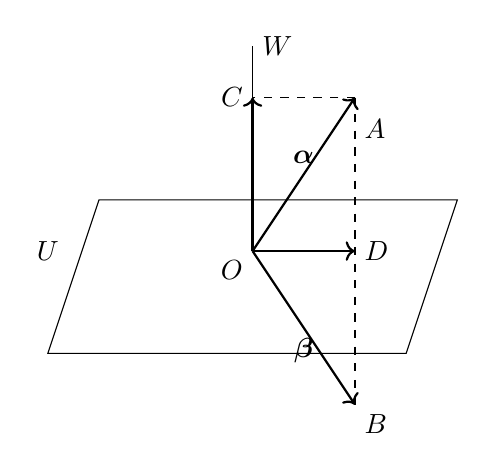
\begin{tikzpicture}[scale=1.3]
		% Define points
		\coordinate (O) at (0,0);
		\coordinate (A) at (1,1.5);
		\coordinate (B) at (1,-1.5);
		\coordinate (C) at (0,1.5);
		\coordinate (D) at (1,0);
		\coordinate (W) at (0,2);
		
		% Draw plane U
		\draw (-2,-1) -- (1.5,-1) -- (2,0.5) -- (-1.5,0.5) -- cycle;
		\node at (-2,0) {$U$};
		
		% Draw vectors
		\draw[thick,->] (O) -- (A) node[midway,above] {$\bm{\alpha}$};
		\draw[thick,->] (O) -- (B) node[midway,below] {$\bm{\beta}$};
		\draw[thick,->] (O) -- (C) node[midway,left] {};
		\draw[thick,->] (O) -- (D) node[midway,below] {};
		\draw[-] (O) -- (W) node[midway,below] {};
		
		% Draw dashed lines
		\draw[dashed] (A) -- (B);
		\draw[dashed] (A) -- (C);
		
		% Label points
		\node at (0,0) [below left] {$O$};
		\node at (1,1) [above right] {$A$};
		\node at (1,-1.5) [below right] {$B$};
		\node at (0,1.5) [left] {$C$};
		\node at (1,0) [right] {$D$};
		\node at (0,2) [right] {$W$};
	\end{tikzpicture}
	\caption{镜面反射示意图}
	\label{fig:reflection}
\end{figure}

如图\ref{fig:reflection},向量 $\overrightarrow{OA}$ 可以分解成 $\overrightarrow{OA} = \overrightarrow{OD} + \overrightarrow{OC}$,其中 $\overrightarrow{OC}$ 与平面 $U$ 垂直,把直线 $\overrightarrow{OC}$ 记作 $W$,它是 $V$ 的一个子空间,且 $V = U \oplus V$. 于是 $\overrightarrow{OC}$ 是 $\bm{\alpha}$ 在投影 $\mathcal{P}_{V}$ 下的像,即
\[
\overrightarrow{OC} = \mathcal{P}_{V}(\bm{\alpha}). 
\]
由于
\[
\bm{\beta} = \overrightarrow{OB} = \overrightarrow{OA} + 2\overrightarrow{AD} = \overrightarrow{OA} + 2(-\overrightarrow{OC}) = \bm{\alpha} - 2\mathcal{P}_{V}(\bm{\alpha}) = (\bm{I} - 2\mathcal{P}_{V})(\bm{\alpha}),
\]
因此 $\mathcal{R}_{U}(\bm{\alpha}) = (\bm{I} - 2\mathcal{P}_{V})\bm{\alpha}, \forall \bm{\alpha} \in V$,从而$
\mathcal{R}_{U} = \bm{I} - 2\mathcal{P}_{V},$
即关于平面 $U$ 的镜面反射 $\mathcal{R}_{U}$ 等于恒等变换 $\bm{I}$ 减去在与平面 $U$ 垂直的直线 $\overline{OC}$ 上的投影 $\mathcal{P}_{V}$ 的 2 倍所得的差.
\begin{definition}{对合变换}{}\kaishu 
	域 $F$ 上线性空间 $V$ 上的线性变换 $\mathcal{A}$ 若满足 $\mathcal{A}^2 = \mathcal{I}$,
	则称 $\mathcal{A}$ 是对合变换. 
\end{definition}
对于几何空间 $ V $ 中任一向量 $\overrightarrow{OA}$ 都有$\mathcal{R}_U^2(\overrightarrow{OA})=\mathcal{R}_U(\overrightarrow{OB}) = \overrightarrow{OA},$于是 $\mathcal{R}_U^i = I$,这就表明几何空间中的镜面反射 $\mathcal{R}_v$ 是一个\textbf{对合变换}. 

在 $\mathbb R[x]_n$ 中,给定 $a \in R$,令
\[
\mathcal{I}_a : \mathbb R[x]_n \longrightarrow R[x]_n,\quad f(x) \longmapsto f(x+a),
\]
由于 $\deg f(x+a) = \deg f(x)$,因此 $\mathcal{I}_a$ 是 $\mathbb R[x]_n$ 到自身的一个映射. 由于 $x$ 用 $x+a$ 代入是保持加法和乘法运算的,因此 $\mathcal{I}_a$ 保持加法和数乘运算,从而 $\mathcal{I}_a$ 是 $R[x]_n$ 上的一个线性变换,称它是由 $a$ 决定的\textbf{平移}. 由泰勒展开式,有
\begin{align*}
	f(x+a) &= f(x) + af'(x) + \frac{a^2}{2!} f''(x) + \cdots + \frac{a^{n-1}}{(n-1)!} f^{(n-1)}(x)\\&= \mathcal{I}(f(x)) + aD(f(x)) + \frac{a^2}{2!}\mathcal D^2(f(x)) + \cdots + \frac{a^{n-1}}{(n-1)!} D^{n-1}(f(x))\\&= (\bm I + a\mathcal D + \frac{a^2}{2!} \mathcal D^2 + \cdots + \frac{a^{n-1}}{(n-1)!}\mathcal D^{n-1}) f(x),
\end{align*}
因此\begin{equation}\label{translation}
	\mathcal{I}_a = \bm I + a\mathcal D + \frac{a^2}{2!}\mathcal D^2 + \cdots + \frac{a^{n-1}}{(n-1)!} \mathcal D^{n-1}.
\end{equation}
\eqref{translation}式表明:平移 $\mathcal{I}_a$ 是求导数 $D$ 的一个多项式. 

我们发现,$\forall f(x) \in \mathbb R[x]_n$,有 $\mathcal D^n(f(x)) = 0$,从而 $\mathcal D^n = \bm O$. 而$\mathcal D^{n-1}(x^{n-1}) = \mathcal D^{n-2}((n-1)x^{n-2}) = \cdots = (n-1)!$,从而 $\mathcal D^{n-1} \neq \bm O$. 于是当 $1 \leqslant k < n$ 时,$\mathcal D^k \neq \bm O$,此时我们称$\mathcal D$为\textbf{幂零变换}.
\begin{definition}{幂零变换}{}\kaishu 
	设 $\mathcal A$ 是域 $\mathbb F$ 上线性空间 $V$ 上的一个线性变换,如果存在正整数 $k$ 使得 $\mathcal A^k = \bm O$,那么称 $\mathcal A$ 是{\heiti 幂零变换};使得 $\mathcal A^k = \bm O$ 成立的最小正整数 $k$ 称为 $\mathcal A$ 的{\heiti 幂零指数}. 
\end{definition}
\begin{example}{}{}
	设 $\mathcal{A}$ 是域 $\mathbb F$ 上线性空间 $V$ 到 $V'$ 的一个线性映射,$W$ 是 $V$ 的一个子空间,令
	\[
	\mathcal{A}W := \{ \mathcal{A}\bm\beta \mid \bm\beta \in W \},
	\]
	证明:
	\begin{enumerate}
		\item[(1)] $\mathcal{A}W$ 是 $V'$ 的一个子空间;
		\item[(2)] 若 $V$ 是有限维的,则\begin{equation}
			\dim(\mathcal{A}W) + \dim((\text{Ker } \mathcal{A}) \cap W) = \dim(W).
		\end{equation}
	\end{enumerate}
\end{example}
\begin{proof}[第一问的证明]
	由于 $\bm 0 \in W$,因此 $\mathcal{A}(\bm 0) \in \mathcal{A}W$. 对于任意 $\bm\alpha, \bm\beta \in W, k \in \mathbb F$,有
	\[
	\mathcal{A}\bm\alpha + \mathcal{A}\bm\beta = \mathcal{A}(\bm\alpha + \bm\beta) \in \mathcal{A}W, \quad k\mathcal{A}\bm\alpha = \mathcal{A}(k\bm\alpha) \in \mathcal{A}W,
	\]
	因此 $\mathcal{A}W$ 是 $V'$ 的一个子空间. 
\end{proof}
\begin{proof}[第二问的证明]
	考虑 $\mathcal{A}$ 在子空间 $W$ 上的限制:$\mathcal{A}\mid W$,它是 $W$ 到 $\mathcal{A}W$ 的一个线性映射. 由于
	\[
	\bm\alpha \in \text{Ker}(\mathcal{A}\mid W) \iff (\mathcal{A}\mid W)\bm\alpha = \bm 0 \iff \mathcal{A}\bm\alpha = \bm 0 \text{且} \bm\alpha \in W \iff \bm\alpha \in (\text{Ker } \mathcal{A}) \cap W,
	\]
	因此
	\[
	\text{Ker}(\mathcal{A}\mid W) = (\text{Ker } \mathcal{A}) \cap W.
	\]
	又显然有 $\text{Im}(\mathcal{A}\mid W) = \mathcal{A}W$,因此
	\[
	\dim(\mathcal{A}W) + \dim((\text{Ker } \mathcal{A}) \cap W) = \dim(W).\qedhere
	\]
\end{proof}
\begin{example}{}{example2.10}
	设 $V, U, W$ 都是域 $F$ 上的线性空间,并且 $V$ 是有限维的. 设 $\mathcal{A} \in \mathcal{L}(V, U)$,$\mathcal{B} \in \mathcal{L}(U, W)$. 证明:
	\begin{equation}\label{example2.10}
		\dim(\text{Ker } \mathcal{BA}) \leqslant \dim(\text{Ker } \mathcal{A}) + \dim(\text{Ker } \mathcal{B}). 
	\end{equation}
\end{example}
\begin{proof}
	首先$\mathcal{BA} \in \mathcal{L}(V, W),\mathcal{BA}V = \mathcal{B}(\mathcal{A}V) = \text{Im}(\mathcal{B}\mid {\mathcal{A}V}), \text{Ker}(\mathcal{B}\mid {\mathcal{A}V}) \subseteq \text{Ker } \mathcal{B}$. 根据线性映射维数公式\ref{thm:dimension of ker and image}得\begin{align*}
		\dim(\text{Ker } \mathcal{BA}) &= \dim V - \dim((\mathcal{BA})V) \\&= \dim V - \dim(\text{Im}(\mathcal{B}\mid{\mathcal{A}V})) \\
		&= \dim V - [\dim(\mathcal{A}V) - \dim(\text{Ker}(\mathcal{B}\mid {\mathcal{A}V}))] \\
		&= \dim V - \dim(\mathcal{A}V) + \dim(\text{Ker}(\mathcal{B}\mid{\mathcal{A}V})) \\
		&\leqslant \dim(\text{Ker } \mathcal{A}) + \dim(\text{Ker } \mathcal{B}).\qedhere
	\end{align*}
\end{proof}
\begin{example}{矩阵秩的Sylvester不等式}{}
	设 $V, U, W$ 都是域 $\mathbb F$ 上的线性空间,并且 $\dim V = n, \dim U = m$. 设 $\mathcal{A} \in \mathcal (V, U), \mathcal{B} \in \mathcal L(U, W)$. 证明:
	\begin{equation}
		\text{rank}(\mathcal{BA}) \geqslant \text{rank}(\mathcal{A}) + \text{rank}(\mathcal{B}) - m. 
	\end{equation}
\end{example}
\begin{proof}
	根据线性映射维数公式\ref{thm:dimension of ker and image}以及例\ref{ex:example2.10}的公式\eqref{example2.10}得
	\begin{align*}
		\text{rank}(\mathcal{BA}) &= \dim(\text{Im}(\mathcal{BA})) \\
		&= \dim V - \dim(\text{Ker}(\mathcal{BA})) \\
		&\geqslant n - [\dim(\text{Ker } \mathcal{A}) + \dim(\text{Ker } \mathcal{B})] \\
		&= n - \dim(\text{Ker } \mathcal{A}) + m - \dim(\text{Ker } \mathcal{B}) - m \\
		&= \dim(\text{Im } \mathcal{A}) + \dim(\text{Im } \mathcal{B}) - m \\
		&= \text{rank}(\mathcal{A}) + \text{rank}(\mathcal{B}) - m.\qedhere
	\end{align*}
\end{proof}
\subsubsection{同态}\label{section:homomorphism}
\begin{definition}{群同态}{group homomorphism}\kaishu 
	设 $G$ 和 $G'$ 是两个群,如果映射 $f: G \to G'$ 满足
	\begin{equation}\label{group homomorphism}
		f(ab) = f(a)f(b), \quad \forall a, b \in G,
	\end{equation}
	则称 $f$ 是 $G$ 到 $G'$ 的一个{\heiti 群同态}. 若对任意 $a \in G$, $f(a) = e'$, 则称 $f$ 是{\heiti 平凡同态}. 若同态 $f$ 是单(满)射,则称 $f$ 是{\heiti 单同态}({\heiti 满同态}). 
	
	若同态 $f$ 是双射,则称 $f$ 是 $G$ 到 $G'$ 的一个{\heiti 群同构},此时称群 $G$ 与 $G'$ 是{\heiti 同构的},记为 $G \cong G'$. 特别地,称群 $G$ 到自身的群同态(或群同构)为 $G$ 的一个{\heiti 自同态}(或{\heiti 自同构}). 
\end{definition}
在式子\eqref{group homomorphism}中,令 $a = b = e$,则易见 $f(e) = e'$;令 $b = a^{-1}$,则可得 $f(a^{-1}) = f(a)^{-1}$. 

可以看出,这里的群同构的定义与线性空间的定义类似,相当于线性空间中“同构”这一概念的推广,事实上,如果只考虑加法,线性空间其实就是一个Abel群,线性空间之间的线性映射保持加法,也就是保持群的运算. 同构之所以重要,因为它保持了所研究的对象——线性空间的代数运算(加法和数乘),从而我们可以得到那些表面不同的线性空间的内在联系. 有些表面上看起来完全不同的线性空间,本质上却是一样的(即它们之间存在线性同构). 类似的保持代数结构的映射是代数学研究中的重要工具,这里我们引入了比同构略弱化的条件,同态. 事实上有群同态和环同态,我们将会从定义看出,同态保持了所研究对象的代数结构. 

与前面完全类似地,我们有
\begin{proposition}{}{group homomorphism}
	若 $f: G_1 \to G_2$, $g: G_2 \to G_3$ 是群同态(单、满或同构),则 $gf: G_1 \to G_3$ 也是群同态(单、满或同构). 特别地,若 $f$ 是同构,则 $f^{-1}$ 也是同构. 
\end{proposition}
\begin{definition}{}{}\kaishu 
	记 $G$ 的自同态的全体为 $\text{Hom}(G)$,自同构的全体为 $\text{Aut}(G)$,则上述命题\ref{pro:group homomorphism}说明 $\text{Hom}(G)$ 是一个幺半群\footnote{定义了满足结合律的乘法的集合是半群,含有幺元的半群称为含幺群,幺元即$ae=a$或$ea=a$的$e$.},而 $\text{Aut}(G)$ 构成群,称为 $G$ 的自同构群. 
\end{definition}
\begin{theorem}{群同态基本定理}{group homomorphism}
	$f: G \to G'$ 是群的满同态,则 $G / \text{Ker} \, f \cong G'$. 
\end{theorem}
这里$G/\mathrm{Ker} f$是商群,与商空间的定义是类似的. 该定理的证明略去,请参考\cite{6}.

最后,我们简单引入环的定义和环同态的概念. 
\begin{definition}{环}{ring}\kaishu 
	设 $R$ 是一个非空集合,如果在 $R$ 中有两种二元运算,且满足下面的条件:
	\begin{enumerate}
		\item $R$ 对于其中一种运算(用加法表示)成为一个交换群,即 $\{R; +\}$ 满足下列条件:
		\begin{enumerate}
			\item $R$ 对运算 “+” 封闭;
			\item 对任何 $a, b, c \in R$,$(a+b)+c = a+(b+c)$,$a+b = b+a$;
			\item $R$ 中存在对 “+” 的单位元,写成零元 $0$,使得 $a+0 = a$,$\forall a \in R$;
			\item 对任何 $a \in R$,存在 $a'$ 使得 $a + a' = 0$. 将 $a'$ 记为 $-a$,称为 $a$ 的负元. 
		\end{enumerate}
		\item $R$ 对于另外一种运算(用乘法表示)成为半群,即对任何 $a, b, c \in R$,有$(ab)c = a(bc).$
		\item $R$ 对于上述两种运算满足下列两条分配律:
		\[
		a(b+c) = ab + ac, \quad (a+b)c = ac + bc, \quad \forall a, b, c \in R,
		\]
	\end{enumerate}
	则称 $R$ 为一个{\heiti 环}. 有时为了更加清楚,也说 $\{R; +, \cdot\}$ 为一个环,其中 “$\cdot$” 为乘法. 
\end{definition}
我们注意到,环的定义中要求对于加法成为交换群,而对另外一种运算只要求成为半群. 如果一个环对于乘法也有幺元,则称该环为\textbf{幺环}. 如果一个环对于乘法交换,则称该环为\textbf{交换环}. 
\begin{definition}{环同态}{}\kaishu 
	设 $R_1, R_2$ 为两个环,$f$ 为 $R_1$ 到 $R_2$ 的一个映射. 如果对任何 $a, b \in R_1$,都有\begin{equation}
		\begin{cases}
			f(a+b) = f(a) + f(b),\\f(ab) = f(a)f(b),
		\end{cases}
	\end{equation}
	则称 $f$ 为一个{\heiti 同态};若同态 $f$ 是单(满)射,则称 $f$ 为单同态;若 $f$ 为同态且是双射,则称 $f$ 为{\heiti 同构},这时也称环 $R_1$ 与 $R_2$ 同构,记为 $R_1 \cong R_2$. 
\end{definition}
我们注意到,环同态 $f$ 是加法群 $R_1$ 到 $R_2$ 的群同态,因此有\begin{equation*}
	f(0) = 0,\quad f(-a) = -f(a), \forall a \in R_1.
\end{equation*}
下面我们给出几个同态的实例. 首先,作为一个平凡的例子,对任何两个环 $R_1, R_2$,定义 $R_1$ 到 $R_2$ 的映射 $f$ 使得对任何 $a \in R_1$,$f(a) = 0$,则 $f$ 是一个同态,称为\textbf{零同态}. 

再看一个高等代数的例子:\begin{example}{}{}
	设 $V$ 为数域 $\mathbb{P}$ 上的 $n$ 维线性空间,$\text{End} \, (V)$ 为 $V$ 上所有线性变换的集合. 容易验证 $\text{End} \, V$ 对于线性变换的加法和乘法构成一个环. 
	
	我们指出,在\ref{liner-map-matrix}中我们构造了线性映射$\mathcal{A}$ 在给定基下的矩阵$\bm A$,并定义了映射$\bm T(\mathcal A):\mathrm{End}(V)\to\mathbb K^{n\times n}$,它是一个同构映射,因而是环$\mathrm{End}(V)$到矩阵环的同构. 
\end{example}

\subsection{线性映射的像与核}\label{image and kernal}
\begin{definition}{线性映射的像与核}{im and ker}\kaishu 
	设 $\mathcal A$ 是数域 $\mathbb{K}$ 上线性空间 $V$ 到 $U$ 的线性映射,$\mathcal A$ 的全体像元素组成 $U$ 的子集称为 $\mathcal A$ 的{\heiti 像},记为 $\text{Im} \, \mathcal A$,即$\mathrm{Im}\mathcal A:=\left\{\mathcal{A}(\bm x)\mid \bm x\in V\right\}.$有时也写成$\mathcal{A}(U).$
	
	$V$ 中在 $\mathcal A$ 下映射为零向量的全体向量构成 $V$ 的子集称为 $\mathcal A$ 的{\heiti 核},记为 $\text{Ker} \, \mathcal A$,即$\mathrm{Ker}\mathcal A:=\{\bm x\in V\mid \mathcal A(\bm x)=\bm 0\in U\}.$
\end{definition}
\begin{proposition}{}{}
	设 $\mathcal A$ 是线性空间 $V \rightarrow U$ 的线性映射,则 $\text{Im} \, \mathcal A$ 是 $U$ 的子空间,$\text{Ker} \, \mathcal A$ 是 $V$ 的子空间. 
\end{proposition}
\begin{proof}
	设 $\bm{\alpha}, \bm\beta \in \text{Im} \, \mathcal A$,则有 $V$ 中向量 $\bm{u}, \bm{v}$,使$\bm{\alpha} = \mathcal A(\bm{u}), \, \bm\beta = \mathcal A(\bm{v}).$
	由于 $\mathcal A(\bm{u} + \bm{v}) = \mathcal A(\bm{u}) + \mathcal A(\bm{v}) = \bm\bm{\alpha} + \bm\beta$,故 $\bm\bm{\alpha} + \bm\beta \in \text{Im} \, \mathcal A$. 若 $k \in \mathbb{K}$,则$\mathcal A(k\bm{u}) = k\mathcal A(\bm{u}) = k\bm{\alpha},$故$k\bm{\alpha} \in \text{Im}\mathcal A. $因此$\text{Im}\mathcal A$是$U$的子空间.

	设 $\bm{u}, \bm{v} \in \text{Ker} \mathcal A$,则 $\mathcal A(\bm{u}) = \mathcal A(\bm{v}) = \bm 0$,从而$\mathcal A(\bm{u} + \bm{v}) = \mathcal A(\bm{u}) + \mathcal A(\bm{v}) = \bm 0,$
	这说明 $\bm{u} + \bm{v} \in \text{Ker}\mathcal A$. 类似地可证明 $k\bm{u} \in \text{Ker}\mathcal A$. 因此 $\text{Ker}\mathcal A$ 是 $V$ 的子空间. 
\end{proof}
\begin{theorem}{}{}
	\begin{enumerate}
		\item[(1)] 线性映射 $\mathcal A$ 是满映射的充分必要条件是 $\dim \text{Im} \mathcal A = \dim U$;
		\item[(2)] 线性映射 $\mathcal A$ 是单映射的充分必要条件是 $\text{Ker} \mathcal A = \bm 0$. 
	\end{enumerate}
\end{theorem}
\begin{proof}
	(1)显然. 下面证明(2).
	
	\textbf{必要性}. 设 $\mathcal{A}$ 是单射,任取 $\alpha \in \text{Ker} \ \mathcal{A}$,则$\mathcal{A}(\bm\alpha) = \bm 0 = \mathcal{A}(\bm 0)$,则 $\bm\alpha = \bm 0$,因此 $\text{Ker} \ \mathcal{A} = \bm 0$. 
	
	\textbf{充分性. }设 $\text{Ker}\mathcal{A} = \bm 0$,设 $\bm\alpha_1, \bm\alpha_2 \in V$,且 $\mathcal{A}(\bm\alpha_1) = \mathcal{A}(\bm\alpha_2)$,则
	\[
	\bm 0 = \mathcal{A}(\alpha_2) - \mathcal{A}(\bm\alpha_1) = \mathcal{A}(\bm\alpha_2 - \bm\alpha_1),
	\]
	从而 $\bm\alpha_2 - \bm\alpha_1 \in \text{Ker} \mathcal{A}$. 由于 $\text{Ker}\mathcal{A} = \bm 0$,故 $\bm\alpha_2 - \bm\alpha_1 = \bm 0$,即 $\bm\alpha_1 = \bm\alpha_2$. 这表明 $\mathcal{A}$ 是单射. 
\end{proof}
\begin{definition}{秩、零度}{rank}\kaishu 
	设 $\mathcal{A}$ 是 $V \rightarrow U$ 的线性映射,像空间 $\text{Im}\mathcal{A}$ 的维数称为 $\mathcal{A}$ 的{\heiti 秩},记作 $\mathrm r(\mathcal{A})$或者$\dim\mathrm{Im}\mathcal A$. 核空间 $\text{Ker}\mathcal{A}$ 的维数称为 $\mathcal{A}$ 的{\heiti 零度}. 
\end{definition}
\begin{definition}{映射的限制}{limitation}\kaishu 
	设 $\bm\varphi: V \rightarrow U$ 为线性映射,$V' \subseteq V, U' \subseteq U$ 为子空间且满足 $\mathrm{Im}\bm\varphi \subseteq U'$,则通过定义域的\textbf{限制}可得线性映射 \[\bm\varphi\mid V': V' \rightarrow U',\quad\bm v\mapsto\bm\varphi(\bm v),\]这样$\bm\varphi\mid V'$ 与 $\bm\varphi$ 具有相同的映射法则. 
\end{definition}
进一步,若 $\bm\varphi$ 是单映射,则 $\bm\varphi\mid V'$ 也是单映射. 
\begin{example}{}{Descartes}
	设 $V$ 是 Descartes 平面,$\mathscr A$ 是绕原点逆时针旋转 $\theta$ 角的线性变换. 
	设 $V'$ 是 $x$-轴所在的一维子空间,$U'$ 是 $\theta$ 角直线所在的一维子空间,则限制映射$\mathscr A\mid V': V' \rightarrow U'$ 不仅是单线性映射,也是满线性映射. 
\end{example}
\begin{theorem}{}{homomorphism theorem}
	设 $\mathcal{A}$ 是域 $\mathbb K$ 上线性空间 $V$ 到 $V'$ 的一个线性映射,令\begin{gather*}
			\sigma: V/\text{Ker}\, \mathcal{A} \longrightarrow \text{Im}\, \mathcal{A}\\\bm\alpha + \text{Ker}\, \mathcal{A} \longmapsto \mathcal{A}\bm\alpha,
	\end{gather*}
	则 $\sigma$ 是 $V/\text{Ker}\, \mathcal{A}$ 到 $\text{Im}\, \mathcal{A}$ 的一个同构映射,从而$V/\text{Ker}\, \mathcal{A} \cong \text{Im}\, \mathcal{A}.$
\end{theorem}
\begin{proof}
	由于
	\[
	\bm\alpha + \text{Ker}\mathcal{A} = \bm\beta + \text{Ker}\mathcal{A}\Longleftrightarrow \bm\alpha - \bm\beta \in \text{Ker}\, \mathcal{A} \quad \Longleftrightarrow \quad \mathcal{A}(\bm\alpha - \bm\beta) = \bm 0 \quad \Longleftrightarrow \quad \mathcal{A}\bm\alpha = \mathcal{A}\bm\beta,
	\]
	因此 $\sigma$是单射,显然$\sigma$ 是满射,因此 $\sigma$ 是双射. 下面验证$\sigma$是线性映射. 
	\begin{align*}
		\sigma[(\bm\alpha + \text{Ker}\, \mathcal{A}) + (\bm\beta + \text{Ker}\, \mathcal{A})] &= \sigma[(\bm\alpha + \bm\beta) + \text{Ker}\, \mathcal{A}] \\&= \mathcal{A}(\bm\alpha + \bm\beta) = \mathcal{A}\bm\alpha + \mathcal{A}\bm\beta,\\&= \sigma(\bm\alpha + \text{Ker}\, \mathcal{A}) + \sigma(\bm\beta + \text{Ker}\, \mathcal{A}),\\
		\sigma[k(\bm\alpha + \text{Ker}\, \mathcal{A})] &= \sigma[k\bm\alpha + \text{Ker}\, \mathcal{A}] \\&= \mathcal{A}(k\bm\alpha) = k\mathcal{A}\bm\alpha	\\&= k\sigma(\bm\alpha + \text{Ker}\, \mathcal{A}).
	\end{align*}
	因此 $\sigma$ 是同构映射,从而 $V/\text{Ker}\, \mathcal{A} \cong \text{Im}\, \mathcal{A}$. 
\end{proof}
\begin{remark}
	本题中的“线性空间”这一条件可以削弱为“群$G$”,即所谓的\textbf{群同态基本定理},请参考前面提到的定理\ref{thm:group homomorphism}. 
\end{remark}
\begin{theorem}{线性映射维数公式}{dimension of ker and image}
	设 $V$ 和 $V'$ 都是域 $\mathbb F$ 上的线性空间,且 $V$ 是有限维的. 设 $\mathcal{A}$ 是 $V$ 到 $V'$ 的一个线性映射,则 $\text{Ker}\, \mathcal{A}$ 和 $\text{Im}\, \mathcal{A}$ 都是有限维的,且
	\[
	\dim(\text{Ker}\, \mathcal{A}) + \dim(\text{Im}\, \mathcal{A}) = \dim V. 
	\]
\end{theorem}
\begin{proof}
	由于 $V$ 有限维,因此 $\text{Ker}\, \mathcal{A}$ 和 $V/\text{Ker}\, \mathcal{A}$ 也是有限维. 从定理\ref{thm:homomorphism theorem}得到 $\text{Im}\, \mathcal{A}$ 也是有限维,且
	\[
	\dim(V/\text{Ker}\, \mathcal{A}) = \dim(\text{Im}\, \mathcal{A}),
	\]
	再由定理\ref{thm:dimension of quotient space}知 $\dim(V) - \dim(\text{Ker}\, \mathcal{A}) = \dim(\text{Im}\, \mathcal{A})$,这就完成了证明. 
\end{proof}
\begin{theorem}{}{}
	设 $V$ 和 $V'$ 都是域 $\mathbb K$ 上 $n$ 维线性空间,且 $\mathcal{A}$ 是 $V$ 到 $V'$ 的一个线性映射,则 $\mathcal{A}$ 是单射当且仅当 $\mathcal{A}$ 是满射. 
\end{theorem}
\begin{proof}
	考虑\begin{align*}
		\mathcal{A}\text{是单射}&\iff\text{Ker}\, \mathcal{A} = \bm 0\\&\iff\dim(\text{Im}\, \mathcal{A}) = \dim(V) = \dim(V')\\&\iff\text{Im}\, \mathcal{A} = V'\\&\iff\mathcal{A} \text{是满射. } \qedhere
	\end{align*}
\end{proof}
由此我们立刻得到一些推论:
\begin{corollary}{}{}
	设 $\mathcal{A}$ 是域 $\mathbb K$ 上有限维线性空间 $V$ 上的一个线性变换,则 $\mathcal{A}$ 是单射$\iff\mathcal{A}$ 是满射. 
\end{corollary}
\begin{corollary}{}{}
	设 $\mathcal{A}$ 是域 $\mathbb K$ 上有限维线性空间 $V$ 上的一个线性变换的充要条件是$\mathcal A$是可逆线性变换. 
\end{corollary}
下面我们继续使用像与核来研究幂等变换和其他的一些重要的线性变换. 
\begin{proposition}{幂等变换就是投影变换}{}
	设 $\mathcal{A}$ 是 $n$ 维线性空间 $V$ 上的幂等变换,证明:$V = U \oplus W$,其中 $U = \text{Im}\,\mathcal{A} = \text{Ker}\bm (\bm I_V - \mathcal{A})$,$W = \text{Im}(\bm I_V - \mathcal{A}) = \text{Ker}\,\mathcal{A}$,且 $\mathcal{A}$ 就是 $V$ 到 $U$ 上的投影变换. 
\end{proposition}
\begin{proof}
	以下简记$V$上的恒等映射$\bm I_V\equiv \bm I.$因为 $\mathcal{A}^2 = \mathcal{A}$,即$\mathcal{A}(\mathcal A-\bm I)=\bm O.$故\begin{equation}
		\text{Im}\,\mathcal{A} \subseteq \text{Ker}(\bm{I} - \mathcal{A}),\quad \text{Im}(\bm{I} - \mathcal{A}) \subseteq \text{Ker}\,\mathcal{A}. 
	\end{equation}对任意的 $\bm{\alpha} \in V$,$\mathcal{A}(\bm{\alpha}) \in \text{Ker}(\bm{I} - \mathcal{A})$,$(\bm{I} - \mathcal{A})(\bm{\alpha}) \in \text{Ker}\,\mathcal{A}$,于是 \[\bm{\alpha} = (\bm{I} - \mathcal{A})(\bm{\alpha}) + \mathcal{A}(\bm{\alpha}) \in \text{Ker}\,\mathcal{A} + \text{Ker}(\bm{I} - \mathcal{A}),\]从而 $V = \text{Ker}\,\mathcal{A} + \text{Ker}(\bm{I} - \mathcal{A})$. 任取 $\bm{\beta} \in \text{Ker}\,\mathcal{A} \cap \text{Ker}(\bm{I} - \mathcal{A})$,则 \[\bm{\beta} = (\bm{I} - \mathcal{A})(\bm{\beta}) + \mathcal{A}(\bm{\beta}) = \bm{0},\]即 $\text{Ker}\,\mathcal{A} \cap \text{Ker}(\bm{I} - \mathcal{A}) = \bm{0}$. 因此,$V = \text{Ker}\,\mathcal{A} \oplus \text{Ker}(\bm{I} - \mathcal{A})$. 特别地,由直和的维数公式\ref{thm:conditions for direct plus}可得 \[\dim \text{Im}\,\mathcal{A} = \dim \text{Ker}(\bm{I} - \mathcal{A}),\quad\dim \text{Im}(\bm{I} - \mathcal{A}) = \dim \text{Ker}\,\mathcal{A},\]从而 $\text{Im}\,\mathcal{A} = \text{Ker}(\bm{I} - \mathcal{A})$,$\text{Im}(\bm{I} - \mathcal{A}) = \text{Ker}\,\mathcal{A}$. 
	
	令 $U = \text{Im}\,\mathcal{A} = \text{Ker}(\bm{I} - \mathcal{A})$,$W = \text{Im}(\bm{I} - \mathcal{A}) = \text{Ker}\,\mathcal{A}$,则 $V = U \oplus W$. 注意到对任意的 $\bm{\alpha} \in V$,$\bm{\alpha} = \mathcal{A}(\bm{\alpha}) + (\bm{I} - \mathcal{A})(\bm{\alpha})$,其中 $\mathcal{A}(\bm{\alpha}) \in U$,$(\bm{I} - \mathcal{A})(\bm{\alpha}) \in W$,结合投影变换的定义\ref{def:project transform},故 $\mathcal{A}$ 就是 $V$ 到 $U$ 上的投影变换. 
\end{proof}

\subsection{线性映射的矩阵表示}\label{liner-map-matrix}
设 $V$ 与 $U$ 分别是数域 $\mathbb{K}$ 上 $n$ 维及 $m$ 维线性空间,$\{\bm{e}_1, \bm{e}_2, \cdots, \bm{e}_n\}$ 是 $V$ 的基,$\{\bm{f}_1, \bm{f}_2, \cdots, \bm{f}_m\}$ 是 $U$ 的基. 又设 $\mathcal{A}$ 是 $V\rightarrow U$ 的线性映射且已知 $V$ 的基向量在 $\mathcal{A}$ 下的像. 若 $V$ 中向量 $\bm{\alpha}$ 在给定基下的坐标向量是 $(\lambda_1, \lambda_2, \cdots, \lambda_n)'$,
设
\begin{equation}\label{represent}
\begin{cases}
	\mathcal{A}(\bm{e}_1) = a_{11}\bm{f}_1 + a_{12}\bm{f}_2 + \cdots + a_{1m}\bm{f}_m, \\
	\mathcal{A}(\bm{e}_2) = a_{21}\bm{f}_1 + a_{22}\bm{f}_2 + \cdots + a_{2m}\bm{f}_m, \\
	\cdots \cdots \\
	\mathcal{A}(\bm{e}_n) = a_{n1}\bm{f}_1 + a_{n2}\bm{f}_2 + \cdots + a_{nm}\bm{f}_m.
\end{cases} 
\end{equation}
因为 $\bm{\alpha} = \lambda_1 \bm{e}_1 + \lambda_2 \bm{e}_2 + \cdots + \lambda_n \bm{e}_n$,简单计算得知 $\mathcal{A}(\bm{\alpha})$ 在 $\{\bm{f}_1, \bm{f}_2, \cdots, \bm{f}_m\}$ 下的坐标向量 $(\mu_1, \mu_2, \cdots, \mu_m)'$ 为
\begin{equation}\label{matrixrepresent}
	\begin{pmatrix}
		\mu_1 \\
		\mu_2 \\
		\vdots \\
		\mu_m
	\end{pmatrix}
	=
	\begin{pmatrix}
		a_{11} & a_{21} & \cdots & a_{n1} \\
		a_{12} & a_{22} & \cdots & a_{n2} \\
		\vdots & \vdots & & \vdots \\
		a_{1m} & a_{2m} & \cdots & a_{nm}
	\end{pmatrix}
	\begin{pmatrix}
		\lambda_1 \\
		\lambda_2 \\
		\vdots \\
		\lambda_n
	\end{pmatrix}.
\end{equation}
上述中的矩阵 $\bm A = (a_{ij})_{m \times n}$ 是 \eqref{represent} 式中系数矩阵的转置. 我们称这个矩阵为 $\mathcal{A}$ 在给定基 $\{\bm{e}_1, \bm{e}_2, \cdots, \bm{e}_n\}$ 与 $\{\bm{f}_1, \bm{f}_2, \cdots, \bm{f}_m\}$ 下的\textbf{表示矩阵},或简称为 $\mathcal{A}$ 在给定基下的矩阵. 

反之,如果 \eqref{matrixrepresent} 式成立,即 $V$ 中向量 $\bm{\alpha}$ 在线性映射 $\mathcal{A}$ 的作用下其坐标向量可以用 \eqref{matrixrepresent} 式来表示,则由 $\bm{e}_1$ 的坐标向量是 $(1, 0, \cdots, 0)'$ 以及 \eqref{matrixrepresent} 式得到 $\mathcal{A}(\bm{e}_1)$ 的坐标向量是 $(a_{11}, a_{12}, \cdots, a_{1m})'$ (即表示矩阵的第一个列向量). 因此
\[
\mathcal{A}(\bm{e}_1) = a_{11}\bm{f}_1 + a_{12}\bm{f}_2 + \cdots + a_{1m}\bm{f}_m.
\]
同理,
\[
\mathcal{A}(\bm{e}_i) = a_{i1}\bm{f}_1 + a_{i2}\bm{f}_2 + \cdots + a_{im}\bm{f}_m.
\]
于是我们得到了 \eqref{represent} 式. 

我们在给定基后,由从 $V$ 到 $U$ 的一个线性映射得到了一个 $m \times n$ 矩阵. 反过来,给定一个 $\mathbb{K}$ 上的 $m \times n$ 矩阵 $\bm A = (a_{ij})_{m\times n}$,由线性扩张定理\ref{thm:Linear extension theorem},我们可以得到 $V\rightarrow U$ 的唯一一个线性映射 $\mathcal{A}$,使 $\mathcal{A}(\bm{e}_i)$ 适合 \eqref{represent} 式. 

若记 $\mathcal{L}(V, U)$ 为从 $V$ 到 $U$ 的线性映射全体组成的集合,$M_{m \times n}(\mathbb{K})$ 是 $\mathbb{K}$ 上 $m \times n$ 矩阵全体组成的集合,则我们得到了一个映射$\bm T:\mathcal{L}(V, U)\longrightarrow M_{m \times n}(\mathbb{K})$,对任意的 $\mathcal{A} \in \mathcal{L}(V, U)$,$\bm T(\mathcal{A}) = A$,其中 $\bm A$ 是 $\mathcal{A}$ 在给定基下的表示矩阵. 前面的分析告诉我们:$\bm T$ 是双射. 

假设 $V$ 的基为 $\{\bm e_1, \bm e_2, \cdots, \bm e_n\}$,$U$ 的基为 $\{\bm f_1, \bm f_2, \cdots, \bm f_m\}$. 记 $\bm \eta_1$ 是 $V$ 到 $\mathbb{K}_n$ 的线性同构;若 $\bm \alpha = a_1\bm e_1 + a_2\bm e_2 + \cdots + a_n\bm e_n$,则$\bm \eta_1(\bm\alpha) = (a_1, a_2, \cdots, a_n)'.$
同样,若 $\bm\beta = b_1\bm f_1 + b_2\bm f_2 + \cdots + b_m\bm f_m$,则令$\bm\eta_2(\bm \beta) = (b_1, b_2, \cdots, b_m)'.$
设 $\bm\varphi \in \mathcal{L}(V, U),\bm T(\bm\varphi) = \bm A$ 是 $\bm\varphi$ 在给定基下的表示矩阵. 我们用 $\bm\varphi$ 表示在例\ref{ex:Matrix multiplication}中定义的从 $\mathbb{K}_n \rightarrow \mathbb{K}_m$ 的线性映射,即若 $\bm x \in \mathbb{K}_n$,则 $\bm\varphi_{\bm A}(\bm x) = \bm{Ax}$. 
\begin{theorem}{建立线性映射与矩阵环的同构}{Linear mapping and matrix}
	设$\bm T$是从$\mathcal{L}(V, U)$到$M_{m \times n}(\mathbb{K})$的线性映射,$\forall \bm\varphi \in \mathcal{L}(V, U),\bm T(\bm\varphi) = \bm A$,则$\bm T$是线性同构,并且$\bm\eta_2\bm\varphi=\bm\varphi_{\bm A}\bm\eta_1,$即有如图\ref{fig:Interchange graph}所示的交换图. 
\end{theorem}
\begin{figure}[h]
	\centering
	\large
	\begin{tikzcd}
		V \arrow[r, "\boldsymbol{\varphi}"] \arrow[d, "\boldsymbol{\eta}_1"] & U \arrow[d, "\boldsymbol{\eta}_2"] \\
		\mathbb K_n \arrow[r, "\boldsymbol{\varphi}_{\boldsymbol A}"]        & \mathbb K_m                       
	\end{tikzcd}
	\caption{}
	\label{fig:Interchange graph}
\end{figure}
\begin{proof}
	我们先验证 $\bm T$ 是一个线性映射. 设 $\bm{\varphi}, \bm\psi$ 是 $V \rightarrow U$ 的线性映射且 $\bm{T}(\bm{\varphi}) = \bm A = (a_{ji}), \bm{T}(\bm\psi) = \bm B = (b_{ji})$. 对任意的 $\bm e_i (i = 1, 2, \cdots, n)$,有
	\[
	(\bm{\varphi} + \bm\psi)(\bm e_i) = \bm{\varphi}(\bm e_i) + \psi(e_i) 
	= \sum_{j=1}^{m} a_{ij}\bm f_j + \sum_{j=1}^{m} b_{ij}\bm f_j 
	= \sum_{j=1}^{m} (a_{ij} + b_{ij})\bm f_j,
	\]
	因此
	\[
	\bm{T}(\bm{\varphi} + \bm \psi) = \bm A + \bm B = \bm{T}(\bm{\varphi}) + \bm{T}(\bm\psi).
	\]
	同理,可证明对任意的 $k \in \mathbb{K}$ 及 $\bm{\varphi} \in \mathcal{L}(V, U)$,有
	\[
	\bm{T}(k\bm{\varphi}) = k\bm A = k\bm{T}(\bm{\varphi}).
	\]
	这表明 $\bm{T}$ 是线性映射. 因为 $\bm{T}$ 是一一对应,故 $\bm{T}$ 是线性同构. 
	要证明图\ref{fig:Interchange graph}所示的交换性,只要对 $V$ 的任一基向量 $\bm e_i$,验证 $\bm\eta_2 \bm\varphi(\bm e_i) = \bm\varphi_{\bm A}\bm\eta_1(\bm e_i)$ 即可. 设
	\[
	\bm A = \begin{pmatrix}
		a_{11} & a_{21} & \cdots & a_{m1} \\
		a_{12} & a_{22} & \cdots & a_{m2} \\
		\vdots & \vdots & & \vdots \\
		a_{1m} & a_{2m} & \cdots & a_{mm}
	\end{pmatrix},
	\]
	则 $\bm\varphi(\bm e_i) = a_{i1}\bm f_1 + a_{i2}\bm f_2 + \cdots + a_{im}\bm f_m$,故
	\[\bm\eta_2 \bm\varphi(\bm e_i) = \begin{pmatrix}
		a_{i1} \\
		a_{i2} \\
		\vdots \\
		a_{im}
	\end{pmatrix}.
	\]
	注意到 $\bm\eta_1(\bm e_i)$ 是第 $i$ 个标准单位列向量,因此 $\bm\varphi_A\bm\eta_1(\bm e_i)$ 就等于 $\bm A$ 的第 $i$ 个列向量,即 $\bm\varphi_{\bm A}\bm\eta_1(\bm e_i) =\bm\eta_2 \bm\varphi(\bm e_i)$,图\ref{fig:Interchange graph}的交换性成立. 
\end{proof}
\begin{theorem}{矩阵乘法的几何意义是线性映射的复合}{}
	同定理\ref{thm:Linear mapping and matrix}的假设,再设 $W$ 是 $\mathbb{K}$ 上的线性空间,$\{\bm g_1, \bm g_2, \cdots, \bm g_p\}$ 是 $W$ 的一组基,$\bm \psi \in \mathcal{L}(U, W)$,则 $\bm T(\bm{\psi \varphi}) = \bm T(\bm\psi)\bm T(\bm\varphi)$. 
\end{theorem}
\begin{proof}
	设 $\bm T(\bm\varphi) = \bm A = (a_{ji})_{m \times n}$,$\bm T(\bm\psi) = \bm B = (b_{kj})_{p \times m}$ 分别是 $\bm\varphi, \bm\psi$ 在给定基下的表示矩阵,又 $\bm\alpha = \lambda_1\bm e_1 + \lambda_2\bm e_2 + \cdots + \lambda_n\bm e_n$ 是 $V$ 中任一向量,则 $\bm\varphi(\bm\alpha)$ 的坐标向量为
	\[(\mu_1,\mu_2,\cdots,\mu_m)^\prime
	= \bm A (\lambda_1,\lambda_2,\cdots,\lambda_n)^\prime,
	\]
	$\bm\psi(\bm\varphi(\bm\alpha))$ 的坐标向量为
	\[(\xi_1,\xi_2,\cdots,\xi_p)'
	= \bm B (\mu_1,\mu_2,\cdots,\mu_m)'.
	\]
	因此
	\[(\xi_1,\xi_2,\cdots,\xi_p)'= \bm{BA} (\lambda_1,\lambda_2,\cdots,\lambda_n)'.\]
	这表明 $\bm T(\bm{\psi\varphi}) = \bm{BA} = \bm T(\bm\psi)\bm T(\bm\varphi).$
\end{proof}
\begin{remark}
	可以看出$\bm T$的作用是\textbf{同态}. 
\end{remark}
由定理不难推出:
\begin{corollary}{}{}
	$\bm T : \mathcal{L}(V) \rightarrow M_n(\mathbb{K})$是线性同构,并对任意的$\bm\varphi, \bm\psi \in \mathcal{L}(V),$ 有
	\[
	\bm T(\bm{\psi \varphi}) = \bm T(\bm\psi)\bm T(\bm \varphi),
	\]
	即 $\bm T$ 保持了乘法. 
\end{corollary}
\begin{proposition}{}{}
	上述同构 $\bm{T}$ 有下列性质:
	\begin{enumerate}
		\item[(1)] $\bm{T}(\bm I_V) = \bm I_n$;
		\item[(2)]	$\bm \varphi$ 是 $V$ 上自同构的充分必要条件是 $\bm{T}(\bm \varphi)$ 为可逆阵且这时有
		\[
		\bm{T}(\bm\varphi^{-1}) = \bm{T}(\bm\varphi)^{-1}.
		\]
	\end{enumerate}
\end{proposition}
\begin{proof}[性质(1)的证明]
	考察 $ V $ 上全体线性变换 $ \mathcal{L}(V) $. 取定 $ V $ 的一组基 $ \{\bm{e}_1, \bm{e}_2, \cdots, \bm{e}_n\} $,对任一 $ \bm{\varphi} \in \mathcal{L}(V) $,设
	\begin{equation}\label{25}
		\begin{cases}
			\bm{\varphi}(\bm{e}_1) = a_{11}\bm{e}_1 + a_{12}\bm{e}_2 + \cdots + a_{1n}\bm{e}_n, \\
			\bm{\varphi}(\bm{e}_2) = a_{21}\bm{e}_1 + a_{22}\bm{e}_2 + \cdots + a_{2n}\bm{e}_n, \\
			\cdots \cdots \cdots \\
			\bm{\varphi}(\bm{e}_n) = a_{n1}\bm{e}_1 + a_{n2}\bm{e}_2 + \cdots + a_{nn}\bm{e}_n,
		\end{cases}
	\end{equation}
	则 $ \bm{\varphi} $ 在基 $ \{\bm{e}_1, \bm{e}_2, \cdots, \bm{e}_n\} $ 下的表示矩阵为 $ n $ 阶方阵 $ \bm A = (a_{ji}) $,即 \eqref{25} 式中系数矩阵的转置,记为 $ \bm T(\bm{\varphi}) = \bm A $. 
	
	当 $\bm\varphi = \bm I_V$ 时\eqref{25} 式中的系数矩阵为 $\bm I_n$,其转置也为 $\bm I_n$,因此结论成立. 
\end{proof}
\begin{proof}[性质(2)的证明]
	由 $\bm{\varphi} \bm{\varphi}^{-1} = \bm I_V$,得
	\[
	\bm{T}(\bm{\varphi})\bm{T}(\bm{\varphi}^{-1}) = \bm{T}(\bm{\varphi} \bm{\varphi}^{-1}) = \bm{T}(\bm I_V) = \bm I_n.
	\]
	此即 $\bm{T}(\bm{\varphi}^{-1}) = \bm{T}(\bm{\varphi})^{-1}$. 充分性也不难验证. 
\end{proof}

上面的这些结论在线性映射与矩阵之间建立起了桥梁,它使我们能用代数的工具(矩阵)来研究几何的对象(线性映射),也能用几何的方法(线性映射)来研究代数的对象(矩阵). 由于线性变换 $ \mathcal{A} $ 与它在 $ V $ 的一个基下的矩阵 $ \bm A $ 的对应是代数同构映射,因此 $ \mathcal L(V) $ 与 $ M_n(\mathbb F) $ 的对应元素之间有关加法、数乘、乘法运算的性质是一样的. 例如,恒等变换 $ \bm I $ 对应于单位矩阵 $ \bm I $;线性变换 $ \mathcal{A} $ 可逆当且仅当它在 $ V $ 的一个基下的矩阵 $ \bm A $ 可逆,且 $ \mathcal{A}^{-1} $ 在 $ V $ 的这个基下的矩阵是 $ \bm A^{-1} $. 

基于这个思想,定理\ref{thm:dimension of ker and image}的矩阵语言版本为\begin{corollary}{}{}
	设$n$维线性空间到$m$维线性空间的线性映射$\mathcal A:V\to U$在给定基下的表示矩阵为$\bm A$,则$\mathcal $是满射的充分必要条件是 $ \text{r}(\bm A) = m $,即表示矩阵 $\bm A $ 是一个行满秩阵;$ \mathcal A $ 是单射的充分必要条件是 $ \text{r}(\bm A) = n $,即 $ \bm A $ 是一个列满秩阵. 
\end{corollary}
\begin{corollary}{}{}
	$ n $ 维线性空间 $ V $ 上的线性变换 $ \mathcal A $ 是单映射(或满映射)的充分必要条件为它在 $ V $ 的任意一组基下的表示矩阵是可逆阵. 
\end{corollary}
事实上,我们还可以看到更多的“等同”关系. 
\begin{theorem}{}{rank rank}
	设 $ \mathcal{A} $ 是域 $ F $ 上 $ n $ 维线性空间 $ V $ 上的线性变换,它在 $ V $ 的一个基 $ \bm\alpha_1, \bm\alpha_2, \cdots, \bm\alpha_n $ 下的矩阵为 $ \bm A $,则	\begin{equation}
		\text{rank}(\mathcal{A})\footnote{注意回忆线性变换的基的定义\ref{def:rank}} = \text{rank}(\bm A).
	\end{equation}
\end{theorem}
\begin{proof}
	由于 $ \mathcal{A}(\bm\alpha) $ 可由 $ \mathcal{A}(\bm\alpha_1), \mathcal{A}(\bm\alpha_2), \cdots, \mathcal{A}(\bm\alpha_n) $ 线性表出,因此
	\[ \text{Im}\mathcal{A} = L\left(\mathcal{A}\alpha_1, \mathcal{A}\alpha_2, \cdots, \mathcal{A}\alpha_n \right). \]
	
	根据表示矩阵\eqref{matrixrepresent}式和命题\ref{pro:1.1},我们知道
	\[ \text{dim}(\text{Im} \mathcal{A}) = \text{dim}L\left(\mathcal{A}\alpha_1, \mathcal{A}\alpha_2, \cdots, \mathcal{A}\alpha_n \right) = \text{rank}(\bm A), \]
	于是
	\[ \text{rank}(\mathcal{A}) = \text{rank}(\bm A).\qedhere \]
\end{proof}
\begin{theorem}{$V$上的线性变换$ \mathcal A$在不同基下的表示矩阵相似}{similar}
	设 $ V $ 是数域 $ \mathbb{K} $ 上的线性空间,$ \mathcal A \in \mathcal{L}(V) $,又设 $ \{\bm{e}_1, \bm{e}_2, \cdots, \bm{e}_n\} $ 及 $ \{\bm{f}_1, \bm{f}_2, \cdots, \bm{f}_n\} $ 是 $ V $ 的两组基且从 $ \{\bm{e}_1, \bm{e}_2, \cdots, \bm{e}_n\} $ 到 $ \{\bm{f}_1, \bm{f}_2, \cdots, \bm{f}_n\} $ 的过渡矩阵为 $ \bm P $. 若 $  \mathcal A $ 在基 $ \{\bm{e}_1, \bm{e}_2, \cdots, \bm{e}_n\} $ 下的表示矩阵为 $ \bm A $,在基 $ \{\bm{f}_1, \bm{f}_2, \cdots, \bm{f}_n\} $ 下的表示矩阵为 $ \bm B $,则$\bm B = \bm P^{-1}\bm{AP}.$
\end{theorem}
\begin{proof}
	设 $ \bm \alpha $ 是 $ V $ 中任一向量且
	\[ \bm\alpha = \lambda_1\bm{e}_1 + \lambda_2\bm{e}_2 + \cdots + \lambda_n\bm{e}_n = \mu_1\bm{f}_1 + \mu_2\bm{f}_2 + \cdots + \mu_n\bm{f}_n, \]
	则由过渡矩阵表示\eqref{transmatrix}式得
	\begin{equation}\label{similar-1}
		\left(\lambda_1,\lambda_2,\cdots,\lambda_n\right)' = \bm P \left(\mu_1,\mu_2,\cdots,\mu_n \right)'.
	\end{equation}
	设\begin{equation}\label{similar-2}
		\mathcal{A}(\bm\alpha) = \xi_1\bm{e}_1 + \xi_2\bm{e}_2 + \cdots + \xi_n\bm{e}_n = \eta_1\bm{f}_1 + \eta_2\bm{f}_2 + \cdots + \eta_n\bm{f}_n,
	\end{equation}
	则由表示矩阵\eqref{matrixrepresent}式得
	\begin{equation}\label{similar-3}
		\begin{pmatrix} \xi_1 \\ \xi_2 \\ \vdots \\ \xi_n \end{pmatrix} = \bm A \begin{pmatrix} \lambda_1 \\ \lambda_2 \\ \vdots \\ \lambda_n \end{pmatrix},\quad \begin{pmatrix} \eta_1 \\ \eta_2 \\ \vdots \\ \eta_n \end{pmatrix} = \bm B \begin{pmatrix} \mu_1 \\ \mu_2 \\ \vdots \\ \mu_n \end{pmatrix}.
	\end{equation}
	另一方面由\eqref{similar-2}式及过渡矩阵的表示\eqref{transmatrix}有\begin{equation}\label{similar-4}
		\begin{pmatrix} \xi_1 \\ \xi_2 \\ \vdots \\ \xi_n \end{pmatrix} = \bm P \begin{pmatrix} \eta_1 \\ \eta_2 \\ \vdots \\ \eta_n \end{pmatrix}.
	\end{equation}
	由\eqref{similar-1}式、\eqref{similar-3}式和\eqref{similar-4}式得\begin{equation}\label{similar-5}
		\bm{PB} \begin{pmatrix} \mu_1 \\ \mu_2 \\ \vdots \\ \mu_n \end{pmatrix} = \bm{AP} \begin{pmatrix} \mu_1 \\ \mu_2 \\ \vdots \\ \mu_n \end{pmatrix}.
	\end{equation}
	但 $ \bm\alpha $ 是任意的,即\eqref{similar-5}式中的 $ \mu_i $ 是任意的,故$\bm{PB}=\bm{AP}$,即$\bm B = \bm P^{-1}\bm{AP}.$
\end{proof}
我们已经看到,$ n $ 维线性空间 $ V $ 上的线性变换与$n$阶方阵有许多相同之处,定理\ref{thm:similar}告诉我们,$ \mathcal{A} $ 在 $ V $ 的不同基下的矩阵是相似的,而 $ n $ 阶方阵的行列式、秩、迹都是相似关系下的不变量,因此我们把 $ \mathcal{A} $ 在 $ V $ 的一个基下的矩阵 $ A $ 的行列式、秩、迹分别叫作线性变换 $ \mathcal{A} $ 的行列式、秩、迹,依次记作 $ \det(\mathcal{A}), \text{rank}(\mathcal{A}), \text{tr}(\mathcal{A}) $. 特别地,定理\ref{thm:rank rank}中指出$ \text{dim}(\text{Im}\mathcal{\bm A}) = \text{rank}(A)=\mathrm{rank}(\mathcal A)$. 

对于 $ n $ 维线性空间 $ V $ 上的线性变换 $ \mathcal{A} $,自然希望在 $ V $ 中找到一个适当的基,使 $ \mathcal{A} $ 在这个基下的矩阵具有最简单的形式,这就相当于给定一个$n$阶矩阵$\bm A$,能否找到一种方法,使得$\bm A$相似于一个比较简单的矩阵. 这就是相似标准形我们要讨论的内容. 

\subsection{不变子空间}
\begin{definition}{不变子空间}{Invariant subspace}\kaishu 
	设 $\mathcal{A}$ 是线性空间 $V$ 上的线性变换,$U$ 是 $V$ 的子空间,若 $U$ 适合条件
	\[
	\mathcal{A}(U) \subseteq U,
	\]
	则称 $U$ 是 $\mathcal{A}$ 的不变子空间(或 $\mathcal{A}$-不变子空间). 这时把 $\mathcal{A}$ 的定义域{\heiti 限制}在 $U$ 上,
	则 $\mathcal{A}$ 在 $U$ 上定义了一个线性变换,称为由 $\mathcal{A}$ {\heiti 诱导}出的线性变换,或称为 $\mathcal{A}$ 在 $U$ 上的{\heiti 限制}\footnote{我们在定义\ref{def:limitation}中已经讲到了这一概念.},记为 $\mathcal{A}\mid U$.
\end{definition}
线性空间 $V$ 上任一线性变换 $\mathcal{A}$ 至少有两个不变子空间:零子空间及全空间 $V$. 因此我们把零子空间及全空间 $V$ 称为\textbf{平凡}的 $\mathcal{A}$-不变子空间. 
\begin{proposition}{}{}
	线性变换 $\mathcal{A}$ 的像与核都是 $\mathcal{A}$ 的不变子空间. 
\end{proposition}
\begin{proof}
	简单验证即可,注意到$\mathcal{A}(\text{Im}\,\mathcal{A}) \subseteq \mathcal{A}(V) = \text{Im}\,\mathcal{A}$, $\mathcal{A}(\text{Ker}\,\mathcal{A}) = \bm 0 \subseteq \text{Ker}\,\mathcal{A}$.
\end{proof}
我们再给出几个例子:\begin{example}{}{}
	Descartes 平面上绕原点的旋转变换$\mathscr A$\footnote{请对比例\ref{ex:Descartes}.},当旋转角 $\theta \neq k\pi$ ($k$ 为整数) 时,没有一维的不变子空间,因此没有非平凡的不变子空间.
\end{example}
\begin{example}{}{}
	设 $\mathcal{A}$ 是 $V$ 上的数乘变换,即存在常数 $k$,使 $\mathcal{A}(\alpha) = k\alpha$,则 $V$ 的任一子空间都是 $\mathcal{A}$ 的不变子空间.
\end{example}
我们再来看线性变换的不变子空间与该线性变换的表示矩阵之间的关系. 
\begin{theorem}{}{}
	设 $\mathcal{A}$ 是域 $\mathbb F$ 上 $n$ 维线性空间 $V$ 上的一个线性变换,$W$ 是 $\mathcal{A}$ 的一个非平凡的不变子空间,$W$ 中取一个基 $\bm{e}_1, \cdots, \bm{e}_r$,把它扩充成 $V$ 的一个基 $\bm{e}_1, \cdots, \bm{e}_r, \bm{e}_{r+1} \cdots, \bm{e}_n$,则 $\mathcal{A}$ 在此基下的矩阵 $\mathcal{A}$ 为一个分块上三角矩阵
	\[
	\mathcal{A} = \begin{pmatrix}
		\bm{A}_1 & \bm{A}_3 \\
		0 & \bm {A}_2
	\end{pmatrix},
	\]
	其中 $\bm{A}_1$ 是 $\mathcal{A}\mid W$ 在 $W$ 的一个基 $\bm{e}_1, \cdots, \bm{e}_r$ 的矩阵,$\bm{A}_2$ 是 $\mathcal A$ 诱导的商空间 $V/W$ 上的线性变换 $\widetilde{\mathcal{A}}$ 在 $V/W$ 的一个基 $\bm{e}_{r+1} + W, \cdots, \bm{e}_n + W$ 下的矩阵. 
\end{theorem}
\begin{proof}
	由于 $\mathcal{A} \bm{e}_i \in W, i = 1, \cdots, r$,因此
	\begin{align*}
		\mathcal{A}(\bm{e}_1, \cdots, \bm{e}_r, \bm{e}_{r+1}, \cdots, \bm{e}_n) &= (\bm{e}_1, \cdots, \bm{e}_r, \bm{e}_{r+1}, \cdots, \bm{e}_n)
		\begin{pmatrix}
			a_{11} & \cdots & a_{1r} & a_{1,r+1} & \cdots & a_{1n} \\
			\vdots & & \vdots & \vdots & & \vdots \\
			a_{r1} & \cdots & a_{rr} & a_{r,r+1} & \cdots & a_{rn} \\
			0 & & 0 & a_{r+1,r+1} & \cdots & a_{r+1,n} \\
			\vdots & & \vdots & \vdots & & \vdots \\
			0 & & 0 & a_{n,r+1} & \cdots & a_{nn}
		\end{pmatrix}\\&= (\bm{e}_1, \cdots, \bm{e}_r, \bm{e}_{r+1} \cdots, \bm{e}_n)
		\begin{pmatrix}
		\bm{A}_1 & \bm{A}_3 \\
		0 & \bm {A}_2
		\end{pmatrix}.
	\end{align*}
	由此看出
	\[
	(\mathcal{A}\mid W)(\bm{e}_1, \cdots, \bm{e}_r) = (\bm{e}_1, \cdots, \bm{e}_r) \bm{A}_1. 
	\]
	商空间 $V/W$ 的一个基为 $\bm{e}_{r+1} + W, \cdots, \bm{e}_n + W$:\begin{align*}
		\widetilde{\mathcal{A}}(\bm{e}_{r+1} + W) &= \mathcal{A} \bm{e}_{r+1} + W\\&= (a_{1,r+1} \bm{e}_1 + \cdots + a_{r,r+1} \bm{e}_r + a_{r+1,r+1} \bm{e}_{r+1} + \cdots + a_{n,r+1} \bm{e}_n) + W\\&= a_{r+1,r+1} (\bm{e}_{r+1} + W) + \cdots + a_{n,r+1} (\bm{e}_n + W),\\\cdots&\cdots\cdots\\\widetilde{\mathcal{A}}(\bm{a}_n + W) = \mathcal{A} \bm{e}_n + W&= (a_{1n} \bm{e}_1 + \cdots + a_{rn} \bm{e}_r + a_{r+1,n} \bm{e}_{r+1} + \cdots + a_{nn} \bm{e}_n) + W\\&= a_{r+1,n} (\bm{e}_{r+1} + W) + \cdots + a_{nn} (\bm{e}_n + W).
	\end{align*}
	因此 $\widetilde{\mathcal{A}}$ 在 $V/W$ 的一个基 $\bm{e}_{r+1} + W, \cdots, \bm{e}_n + W$ 下的矩阵为
	\[
	\begin{pmatrix}
		a_{r+1,r+1} & \cdots & a_{r+1,n} \\
		\vdots & & \vdots \\
		a_{n,r+1} & \cdots & a_{nn}
	\end{pmatrix}
	= \bm{A}_2. \qedhere
	\]
\end{proof}
\begin{remark}
	引入特征值相关内容后,我们还可以进一步证明:设 $\mathcal{A}, \mathcal{A}\mid W, \tilde{\mathcal{A}}$ 的特征多项式分别为 $f(\lambda), f_1(\lambda), f_2(\lambda)$,则 $f(\lambda) = f_1(\lambda) f_2(\lambda)$. 
\end{remark}
进一步地,可以得到推论:
\begin{corollary}{}{}
	设 $V = V_1 \oplus V_2 \oplus \cdots \oplus V_m$,其中每个 $V_i$ 都是线性变换 $\mathcal{A}$ 的不变子空间,那么在 $V$ 中存在一组基(这组基可由 $V_i$ 的基合并而成),使 $\mathcal{A}$ 在这组基下的表示矩阵为分块对角阵:
	\[
	\begin{pmatrix}
		\bm{A}_1 & & & \\
		& \bm{A}_2 & & \\
		& & \ddots & \\
		& & & \bm{A}_m
	\end{pmatrix},
	\]
	其中 $\mathcal{A}_i$ 是 $\mathcal{A}\mid {V_i}$ 的表示矩阵,它是 $r_i$ 阶方阵,$r_i = \dim V_i$. 
\end{corollary}
如果 $n$ 维线性空间的线性变换 $\mathcal{A}$ 有足够小的不变子空间,比如有 $n$ 个一维不变子空间,其直和正好组成全空间,那么上述中的表示矩阵就是一个对角阵. 
\begin{example}{}{}
	设 $V_1, V_2$ 是 $V$ 上线性变换 $\mathcal{A}$ 的不变子空间,则$V_1 \cap V_2$,$V_1 + V_2$ 也是 $\mathcal{A}$ 的不变子空间. 
\end{example}
\begin{proof}
	取 $\bm{v} \in V_1 \cap V_2$,则由 $\bm{v} \in V_i$ 可得 $\mathcal{A}(\bm{v}) \in V_i (i = 1,2)$,于是 $\mathcal{A}(\bm{v}) \in V_1 \cap V_2$,从而 $V_1 \cap V_2$ 是 $\mathcal{A}$-不变子空间. 
	
	任取 $\bm{v} \in V_1 + V_2$,则 $\bm{v} = \bm{v}_1 + \bm{v}_2$,其中 $\bm{v}_i \in V_i$,故 $\mathcal{A}(\bm{v}_i) \in V_i (i = 1,2)$,于是 $\mathcal{A}(\bm{v}) = \mathcal{A}(\bm{v}_1) + \mathcal{A}(\bm{v}_2) \in V_1 + V_2$,从而 $V_1 + V_2$ 是 $\mathcal{A}$-不变子空间. 
\end{proof}
\begin{example}{}{}
	设 $\mathcal{A}$ 是 $n$ 维线性空间 $V$ 上的自同构,若 $W$ 是 $\mathcal{A}$ 的不变子空间,求证:$W$ 也是 $\mathcal{A}^{-1}$ 的不变子空间. 
\end{example}
\begin{proof}
	将 $\mathcal{A}$ 限制在 $W$ 上,它是 $W$ 上的线性变换. 由于 $\mathcal{A}$ 是单映射,故它在 $W$ 上的限制也是单映射,从而也是满映射,即它是 $W$ 上的自同构,于是 $\mathcal{A}(W) = W$,由此即得 $\mathcal{A}^{-1}(W) = W$. 
\end{proof}
\begin{remark}
	如果 $V$ 是无限维线性空间,则本例的结论一般并不成立. 例如,$V = \mathbb{K}[x^{-1}, x]$ 是由数域 $\mathbb{K}$ 上的 Laurent 多项式 $\displaystyle f(x) = \sum_{i=-m}^{n} a_i x^i (m, n \in \mathbb{N})$ 构成的线性空间,$V$ 上的线性变换 $\mathcal{A}, \mathcal B$ 定义为 $\mathcal{A}(f(x)) = xf(x), \mathcal B(f(x)) = x^{-1}f(x)$. 显然,$\mathcal{A}, \mathcal B$ 互为逆映射,从而都是自同构。注意到 $W = \mathbb{K}[x]$ 是 $V$ 的 $\mathcal{A}$-不变子空间,但 $W$ 显然不是 $\mathcal{A}^{-1}$-不变子空间. 
\end{remark}
\begin{example}{}{2.16}
	设 $\mathcal{A}$ 是 $n (n \geqslant 2)$ 维线性空间 $V$ 上的线性变换,证明以下 $n$ 个结论等价:
	\begin{enumerate}
		\item[(1)] $V$ 的任一 1 维子空间都是 $\mathcal{A}$-不变子空间;
		
		$\cdots\cdots$
		\item[($r$)] $V$ 的任一 $r$ 维子空间都是 $\mathcal{A}$-不变子空间;
		
		$\cdots\cdots$
		\item[($n-1$)] $V$ 的任一 $n-1$ 维子空间都是 $\mathcal{A}$-不变子空间;
		\item[($n$)] $\mathcal{A}$ 是纯量变换.
	\end{enumerate}
\end{example}
\begin{proof}
	注意到当 $1 \leqslant i \leqslant n-2$ 时,任一 $i$ 维子空间 $V_0$ 都可表示为两个 $i+1$ 维子空间 $V_1, V_2$ 的交,于是由例\ref{ex:2.16}可知:$(n) \Longrightarrow (n-1) \Longrightarrow (n-2) \Longrightarrow \cdots \Longrightarrow (1)$ 显然成立,剩下只要证明 $(1) \Longrightarrow (n)$ 即可. 
	
	取 $V$ 的一组基 $\{\bm{e}_1, \bm{e}_2, \cdots, \bm{e}_n\}$,由 (1) 可设 $\mathcal{A}(\bm{e}_i) = \lambda_i \bm{e}_i (1 \leqslant i \leqslant n)$. 只要证明 $\lambda_1 = \lambda_2 = \cdots = \lambda_n$ 即可得到 $\mathcal{A}$ 为纯量变换. 用反证法,不妨设 $\lambda_1 \neq \lambda_2$,则由 $L(\bm{e}_1 + \bm{e}_2)$ 也是 $\mathcal{A}$-不变子空间可设 $\mathcal{A}(\bm{e}_1 + \bm{e}_2) = \lambda_0 (\bm{e}_1 + \bm{e}_2)$,于是 $(\lambda_1 - \lambda_0) \bm{e}_1 + (\lambda_2 - \lambda_0) \bm{e}_2 = \mathbf{0}$,从而 $\lambda_1 = \lambda_2 = \lambda_0$,矛盾. 
\end{proof}
\newpage
\begin{thebibliography}{99}  
	
	\bibitem{1}谢启鸿,姚慕生,吴泉水. 高等代数学(第四版). 上海:复旦大学出版社, 2022.
	\bibitem{2}谢启鸿,姚慕生. 高等代数(第四版). 上海:复旦大学出版社, 2022.
	\bibitem{3}丘维声. 高等代数(第二版,下册). 北京:清华大学出版社, 2018. 
	\bibitem{4}徐森林,胡自胜,金亚东,薛春华. 点集拓扑. 合肥:中国科学技术大学出版社, 2019. 
	\bibitem{5}夏道行, 吴卓人, 严绍宗, 舒五昌. 实变函数论与泛函分析(第二版修订本,上册). 北京:高等教育出版社,2010.  
	\bibitem{6}邓少强,朱富海. 抽象代数. 北京:科学出版社,2017. 
	
\end{thebibliography}
\end{document}
